\appendix

\chapter*{APPENDICES}
\addcontentsline{toc}{chapter}{APPENDICES}

\newcounter{appx}
\renewcommand{\theappx}{\Alph{appx}}
% Appendix-style numbering: Table A.1, Figure A.1, etc.
\renewcommand{\thetable}{\theappx.\arabic{table}}
\renewcommand{\thefigure}{\theappx.\arabic{figure}}

\setcounter{table}{0}\setcounter{figure}{0}
\refstepcounter{appx}\label{app:A}
\section*{Appendix \theappx: Course assessment timeline}
\addcontentsline{toc}{section}{Appendix \theappx: Course assessment timeline}

Table~\ref{tab:full-timeline} presents the complete timeline of seminar assessments with Google Forms links and the number of quiz blocks per seminar, as extracted from the Viber chat log.

\begin{table}[!h]
\centering
\caption{Seminar assessment timeline (complete; see Section~\ref{sec:organisation})}
\label{tab:full-timeline}
\small
\begin{tabular}{clcc}
\hline
\textbf{Sem.} & \textbf{Date} & \textbf{Blocks} & \textbf{Naming theme} \\
\hline
1 & 2024-10-20 & 6 & Numbered (Тест 1--6) \\
2 & 2024-10-27 & 5 & Numbered (Блок 1--5) \\
3 & 2024-11-03 & 3 & Parts (Частина 1--3) \\
4 & 2024-11-10 & 1 & Single form \\
5 & 2024-11-10 & 5 & Numbered (Блок 1--5) \\
6 & 2024-11-17 & 5 & Numbered (Блок 1--5) \\
7 & 2024-11-24 & 4 & Numbered (Блок 1--4) \\
8 & 2024-12-01 & 5 & Roman numerals (І--V) \\
8* & 2024-12-08 & 5 & Parts (Частина 1--5) \\
9 & 2024-11-24 & 5 & Numbered (Блок 1--5) \\
10 & 2024-12-01 & 2 & Lecture-based \\
11 & 2024-12-15 & 5 & Chapter (Chapter 1--5) \\
12 & 2024-12-22 & 7 & Блок 1--5 + Extra 1--2 \\
13 & 2024-12-29 & 1 & Single form \\
14 & 2025-01-05 & 5 & Part 1--5 \\
15 & 2025-01-12 & 4 & Parts (Частина 1--4) \\
16 & 2025-01-19 & 3 & Numbered (Блок 1--3) \\
17 & 2025-01-19 & 5 & Greek alphabet ($\alpha$--$\epsilon$) \\
18 & 2025-01-26 & 3 & Numbered (Блок 1--3) \\
19 & 2025-02-02 & 4 & Gemstones \\
20 & 2025-02-02 & 5 & Greek mythology \\
21 & 2025-02-09 & 5 & Greek alphabet (Ukrainian) \\
22--23 & 2025-02-16 & 6 & Numbered (Блок 1--6) \\
24 & 2025-02-23 & 4 & Numbered (Блок 1--4) \\
25 & 2025-03-02 & 4 & Flowers \\
26 & 2025-03-09 & 4 & Numbered (Блок 1--4) \\
27 & 2025-03-16 & 4 & Trees \\
28 & 2025-03-16 & 5 & Number words \\
29 & 2025-03-23 & 4 & Flowers (repeated) \\
30 & 2025-03-30 & 4 & Minerals \\
31--39 & 2025-04-06--13 & var. & NMT practice formats \\
\hline
\multicolumn{4}{l}{\footnotesize\textit{Note: Seminars 31--39 used NMT examination practice formats;}} \\
\multicolumn{4}{l}{\footnotesize\textit{detailed quiz-block data are reported in Section~\ref{sec:formative}.}} \\
\end{tabular}
\end{table}

\setcounter{table}{0}\setcounter{figure}{0}
\refstepcounter{appx}\label{app:B}
\section*{Appendix \theappx: HistoryLikeGame platform modules}
\addcontentsline{toc}{section}{Appendix \theappx: HistoryLikeGame platform modules}

Table~\ref{tab:game-catalog} lists all interactive game modules available on the HistoryLikeGame platform (current version). Modules marked with~(*) were available during the experimental period (December 2024 -- May 2025).

\begin{small}
\begin{longtable}{@{}>{\raggedright}p{3.0cm}l>{\raggedright}p{2.3cm}>{\raggedright}p{2.2cm}>{\raggedright\arraybackslash}p{3.0cm}@{}}
\caption{Catalogue of HistoryLikeGame modules} \label{tab:game-catalog} \\
\hline
\textbf{Module} & \textbf{Period} & \textbf{Game type} & \textbf{Technology} & \textbf{Description} \\
\hline
\endfirsthead
\multicolumn{5}{l}{\textit{Table~\ref{tab:game-catalog} continued}} \\
\hline
\textbf{Module} & \textbf{Period} & \textbf{Game type} & \textbf{Technology} & \textbf{Description} \\
\hline
\endhead
\hline
\endfoot
Chronobiy & 0 & Timeline battle & Three.js & Sort events chronologically to defeat opponents \\
Block Buster* & 0 & Breakout & Canvas & Arkanoid-style with historical content \\
Compass & 0 & Navigation & Canvas/Map & Interactive compass puzzle \\
Solitaire (intro) & 0 & Card game & Canvas & Introductory solitaire \\
Ancient explorer & 1 & Path builder & Interactive & Explore ancient Ukrainian territories \\
Kyivan Rus quiz* & 2 & Falling-answer & Template & Timed falling-date selection \\
Viking's Gift & 2 & Apple catcher & Canvas & Catch items with Viking character \\
Lithuanian quiz & 3 & Falling-answer & Template & Timed falling-date selection \\
Hist.\ solitaire v2 & 4 & Card game & Canvas & 4-theme chronological sorting \\
Cossack quiz & 4 & Falling-answer & Canvas+JS & Self-contained falling game \\
Bobble Shooter & 5 & Bubble shooter & Canvas & Match 3+ coloured historical categories \\
Tower Defence & 5 & Tower defence & Three.js & 3D fortress defence game \\
Revolution & 6 & Quiz embed & Wordwall & External platform integration \\
Portrait Puzzle & 7 & Drag-drop puzzle & DOM & Assemble portraits of Mazepa, Petliura, Sahaidachny \\
Caf\'{e} simulator & 8 & Simulation & Canvas/DOM & Independence-era caf\'{e} management \\
\hline
\multicolumn{5}{l}{\textit{Christmas special ($\alpha$)~-- deployed during experimental period}} \\
\hline
Crstm\_S\_1\_1--1\_5* & $\alpha$ & Quiz (D\&D+text) & Shared engine & Ancient/Medieval history (7 modules) \\
Crstm\_S\_2\_1--2\_5* & $\alpha$ & Quiz (D\&D+text) & Shared engine & Early modern period (5 modules) \\
Crstm\_S\_3\_1--3\_5* & $\alpha$ & Quiz (D\&D+text) & Shared engine & 19th--early 20th century (5 modules) \\
Crstm\_S\_4\_1--4\_5* & $\alpha$ & Quiz (D\&D+text) & Shared engine & 20th century (5 modules) \\
Crstm\_S\_Omega* & $\alpha$ & Quiz (text) & Shared engine & Comprehensive review (1 module) \\
\hline
\multicolumn{5}{l}{\textit{Augmented Reality section~-- not deployed during experiment;}} \\
\multicolumn{5}{l}{\textit{designed for future use with specialised students}} \\
\hline
Quebec AR & AR & 3D scene & A-Frame+AR.js & Desktop and mobile AR variants \\
Toronto AR & AR & 3D scene & A-Frame & Virtual historical exploration \\
Yukon AR & AR & 3D textbook & A-Frame+AR.js & Civic education; 5 colour-coded variants (pseudonymised per student, structurally identical) \\
\hline
\multicolumn{5}{l}{\textit{Additional}} \\
\hline
Mini-game ($\beta$) & $\beta$ & Inline puzzle & DOM & 3$\times$3 sliding puzzle (50\% random) \\
Historical map & -- & Interactive map & DOM & De Boplan historical map exploration \\
\hline
\end{longtable}
\end{small}

\setcounter{table}{0}\setcounter{figure}{0}
\refstepcounter{appx}\label{app:C}
\section*{Appendix \theappx: List of applicant's publications on the dissertation topic}
\addcontentsline{toc}{section}{Appendix \theappx: List of applicant's publications on the dissertation topic}

\printpratsi

\setcounter{table}{0}\setcounter{figure}{0}
\refstepcounter{appx}\label{app:D}
\section*{Appendix \theappx: Approbation of dissertation results}
\addcontentsline{toc}{section}{Appendix \theappx: Approbation of dissertation results}

\printconf

\setcounter{table}{0}\setcounter{figure}{0}
\refstepcounter{appx}\label{app:E}
\section*{Appendix \theappx: Data analysis pipeline}
\addcontentsline{toc}{section}{Appendix \theappx: Data analysis pipeline}

The complete source code for the data analysis pipeline is available in the \texttt{thesis/analysis/} directory and consists of the following modules:

\begin{enumerate}
\item \texttt{parse\_chat.py} -- Chat log parser (400 messages processed)
\item \texttt{extract\_assessments.py} -- Assessment timeline extractor (156 forms catalogued)
\item \texttt{analyze\_responses.py} -- Google Forms response analyser (36 seminars, 90 named participants)
\item \texttt{track\_attendance.py} -- Attendance and enrollment tracker (23 participants, 33 absences)
\item \texttt{catalog\_gamification.py} -- Gamification platform cataloguer (62 modules)
\item \texttt{generate\_figures.py} -- Publication figure generator
\item \texttt{run\_pipeline.py} -- Master pipeline orchestrator
\end{enumerate}

\setcounter{table}{0}\setcounter{figure}{0}
\refstepcounter{appx}\label{app:F}
\section*{Appendix \theappx: Supplementary figures and tables}
\addcontentsline{toc}{section}{Appendix \theappx: Supplementary figures and tables}

The following figures and tables provide supplementary detail for the analyses presented in the main text. Each item includes a back-reference to the relevant section.

% --- Chapter 1 supplementary figures ---

\begin{figure}[!h]
\centering
\begin{tikzpicture}
\begin{axis}[
  width=\textwidth,
  height=13cm,
  date coordinates in=x,
  xticklabel={\year},
  xtick={1960-01-01, 1970-01-01, 1980-01-01, 1990-01-01, 2000-01-01, 2010-01-01, 2020-01-01},
  xticklabel style={font=\small},
  xmin=1958-01-01, xmax=2028-01-01,
  ymin=-2.2, ymax=3.0,
  ytick=\empty,
  axis x line=middle,
  axis y line=none,
  x axis line style={->, thick, gray!70},
  enlarge x limits=0.01,
  clip=false
]

% === Era background shading ===
\fill[blue!6] (axis cs:1958-01-01,-2.2) rectangle (axis cs:1990-01-01,3.0);
\fill[red!5] (axis cs:1990-01-01,-2.2) rectangle (axis cs:2008-06-01,3.0);
\fill[green!5] (axis cs:2008-06-01,-2.2) rectangle (axis cs:2018-06-01,3.0);
\fill[orange!5] (axis cs:2018-06-01,-2.2) rectangle (axis cs:2028-01-01,3.0);

% === Era labels — top, left-aligned within each band ===
\node[font=\footnotesize\itshape, blue!70!black, anchor=west] at (axis cs:1959-01-01,2.75) {Cliometrics era};
\node[font=\footnotesize\itshape, red!70!black, anchor=west] at (axis cs:1991-01-01,2.75) {CHNM founding era};
\node[font=\footnotesize\itshape, green!50!black, anchor=west] at (axis cs:2009-01-01,2.75) {DH expansion};
\node[font=\footnotesize\itshape, orange!70!black, anchor=west] at (axis cs:2019-01-01,2.75) {Pedagogical turn};

% === Thin vertical era dividers ===
\draw[dashed, gray!30] (axis cs:1990-01-01,-2.2) -- (axis cs:1990-01-01,2.55);
\draw[dashed, gray!30] (axis cs:2008-06-01,-2.2) -- (axis cs:2008-06-01,2.55);
\draw[dashed, gray!30] (axis cs:2018-06-01,-2.2) -- (axis cs:2018-06-01,2.55);

% === Milestone dots on axis ===
\addplot[only marks, mark=*, mark size=4pt, blue!80!black] coordinates {(1964-01-01,0)};
\addplot[only marks, mark=*, mark size=4pt, blue!80!black] coordinates {(1974-01-01,0)};
\addplot[only marks, mark=square*, mark size=4pt, red!70!black] coordinates {(1994-01-01,0)};
\addplot[only marks, mark=square*, mark size=4pt, red!70!black] coordinates {(2006-01-01,0)};
\addplot[only marks, mark=triangle*, mark size=4.5pt, green!60!black] coordinates {(2012-01-01,0)};
\addplot[only marks, mark=triangle*, mark size=4.5pt, green!60!black] coordinates {(2015-06-01,0)};
\addplot[only marks, mark=diamond*, mark size=4.5pt, orange!80!black] coordinates {(2020-01-01,0)};
\addplot[only marks, mark=diamond*, mark size=4.5pt, orange!80!black] coordinates {(2022-01-01,0)};
\addplot[only marks, mark=pentagon*, mark size=5.5pt, black, fill=black!70] coordinates {(2025-06-01,0)};

% ==================================================================
% ABOVE the axis — 3 levels: 0.5, 1.2, 1.9
% Each level has entries spaced >= 20 years apart to avoid overlap.
%
%   Level 1.9:  1964                                         2025
%   Level 1.2:                            2012
%   Level 0.5:            1994                      2020
% ==================================================================

% 1964 — level 1.9 (top)
\draw[thin, gray!50] (axis cs:1964-01-01,0) -- (axis cs:1964-01-01,1.9);
\node[above, text width=2.5cm, align=center, font=\scriptsize]
  at (axis cs:1964-01-01,1.9) {1964\\Cliometrics\\(Fogel)};

% 1994 — level 0.5 (low)
\draw[thin, gray!50] (axis cs:1994-01-01,0) -- (axis cs:1994-01-01,0.5);
\node[above, text width=2.8cm, align=center, font=\scriptsize]
  at (axis cs:1994-01-01,0.5) {1994\\H-Net /\\Valley of the Shadow};

% 2012 — level 1.2 (mid)
\draw[thin, gray!50] (axis cs:2012-01-01,0) -- (axis cs:2012-01-01,1.2);
\node[above, text width=2.5cm, align=center, font=\scriptsize]
  at (axis cs:2012-01-01,1.2) {2012\\Computational\\Turn (Berry)};

% 2020 — level 0.5 (low), 26 years from 1994
\draw[thin, gray!50] (axis cs:2020-01-01,0) -- (axis cs:2020-01-01,0.5);
\node[above, text width=2.8cm, align=center, font=\scriptsize]
  at (axis cs:2020-01-01,0.5) {2020\\State of the Field\\(Romein et al.)};

% 2025 — level 1.9 (top), 61 years from 1964
\draw[thin, gray!50] (axis cs:2025-06-01,0) -- (axis cs:2025-06-01,1.9);
\node[above, text width=2.5cm, align=center, font=\scriptsize\bfseries]
  at (axis cs:2025-06-01,1.9) {2025\\This\\dissertation};

% ==================================================================
% BELOW the axis — 3 levels: -0.5, -1.2, -1.9
%
%   Level -0.5:   1974                          2015
%   Level -1.2:                  2006                       2022
%   Level -1.9:   (empty)
% ==================================================================

% 1974 — level -0.5 (shallow)
\draw[thin, gray!50] (axis cs:1974-01-01,0) -- (axis cs:1974-01-01,-0.5);
\node[below, text width=2.8cm, align=center, font=\scriptsize]
  at (axis cs:1974-01-01,-0.5) {1974\\\textit{Time on the Cross}\\(Fogel \& Engerman)};

% 2006 — level -1.2 (deep)
\draw[thin, gray!50] (axis cs:2006-01-01,0) -- (axis cs:2006-01-01,-1.2);
\node[below, text width=3cm, align=center, font=\scriptsize]
  at (axis cs:2006-01-01,-1.2) {2006\\\textit{Digital History}\\(Cohen \& Rosenzweig)};

% 2015 — level -0.5 (shallow), 41 years from 1974
\draw[thin, gray!50] (axis cs:2015-06-01,0) -- (axis cs:2015-06-01,-0.5);
\node[below, text width=2.8cm, align=center, font=\scriptsize]
  at (axis cs:2015-06-01,-0.5) {2015\\Historian's Macroscope\\(Graham et al.)};

% 2022 — level -1.2 (deep), 16 years from 2006
\draw[thin, gray!50] (axis cs:2022-01-01,0) -- (axis cs:2022-01-01,-1.2);
\node[below, text width=2.5cm, align=center, font=\scriptsize]
  at (axis cs:2022-01-01,-1.2) {2022\\DH Primer\\(Guiliano)};

\end{axis}
\end{tikzpicture}

\caption{Evolution of digital history: from cliometrics to pedagogical turn (1964--2025) (see Section~\ref{sec:dh-review}).}
\label{fig:dh-timeline}
\end{figure}

\begin{figure}[!h]
\centering
\begin{tikzpicture}
  % Larger geometry: circles further apart with bigger radius
  \def\radius{3.5cm}
  \def\sep{2.0cm}
  \coordinate (H) at (90:\sep);   % History — top
  \coordinate (D) at (210:\sep);  % Digital Humanities — bottom left
  \coordinate (P) at (330:\sep);  % Pedagogy — bottom right

  % Draw filled circles with transparency
  \begin{scope}[opacity=0.12]
    \fill[blue] (H) circle (\radius);
    \fill[red] (D) circle (\radius);
    \fill[green!70!black] (P) circle (\radius);
  \end{scope}

  % Draw circle outlines
  \draw[thick, blue!80!black] (H) circle (\radius);
  \draw[thick, red!80!black] (D) circle (\radius);
  \draw[thick, green!60!black] (P) circle (\radius);

  % Main domain labels (outside circles, pushed further out)
  \node[font=\bfseries, blue!80!black] at (90:5.2cm)
    {\begin{tabular}{c}History\\[-2pt]\scriptsize\textit{historical thinking,}\\[-3pt]\scriptsize\textit{source analysis,}\\[-3pt]\scriptsize\textit{disciplinary knowledge}\end{tabular}};
  \node[font=\bfseries, red!80!black] at (210:5.4cm)
    {\begin{tabular}{c}Digital\\Humanities\\[-2pt]\scriptsize\textit{computational methods,}\\[-3pt]\scriptsize\textit{digital tools, data literacy}\end{tabular}};
  \node[font=\bfseries, green!60!black] at (330:5.4cm)
    {\begin{tabular}{c}Pedagogy\\[-2pt]\scriptsize\textit{learning theories,}\\[-3pt]\scriptsize\textit{assessment,}\\[-3pt]\scriptsize\textit{instructional design}\end{tabular}};

  % Pairwise intersection labels — pushed deep into outer petals
  % History ∩ DH = "Digital History (research)" — upper-left petal
  \node[font=\small\itshape, text width=2.4cm, align=center]
    at ($(H)!0.5!(D) + (150:1.8cm)$) {Digital History\\(research)};

  % History ∩ Pedagogy = "History Education" — upper-right petal
  \node[font=\small\itshape, text width=2.4cm, align=center]
    at ($(H)!0.5!(P) + (30:1.8cm)$) {History\\Education};

  % DH ∩ Pedagogy = "Digital Pedagogy" — bottom petal
  \node[font=\small\itshape, text width=2.4cm, align=center]
    at ($(D)!0.5!(P) + (270:1.8cm)$) {Digital\\Pedagogy};

  % Central triple intersection — the thesis focus
  \node[font=\bfseries\small, text width=2.6cm, align=center,
        fill=yellow!30, rounded corners=3pt, inner sep=4pt,
        draw=yellow!60!black, thin]
    at (0,0) {Digital History\\Pedagogy};
\end{tikzpicture}

\caption{Digital history pedagogy as the intersection of three scholarly domains (see Section~\ref{sec:dh-review}).}
\label{fig:dh-venn}
\end{figure}

\begin{figure}[!h]
\centering
\resizebox{\textwidth}{!}{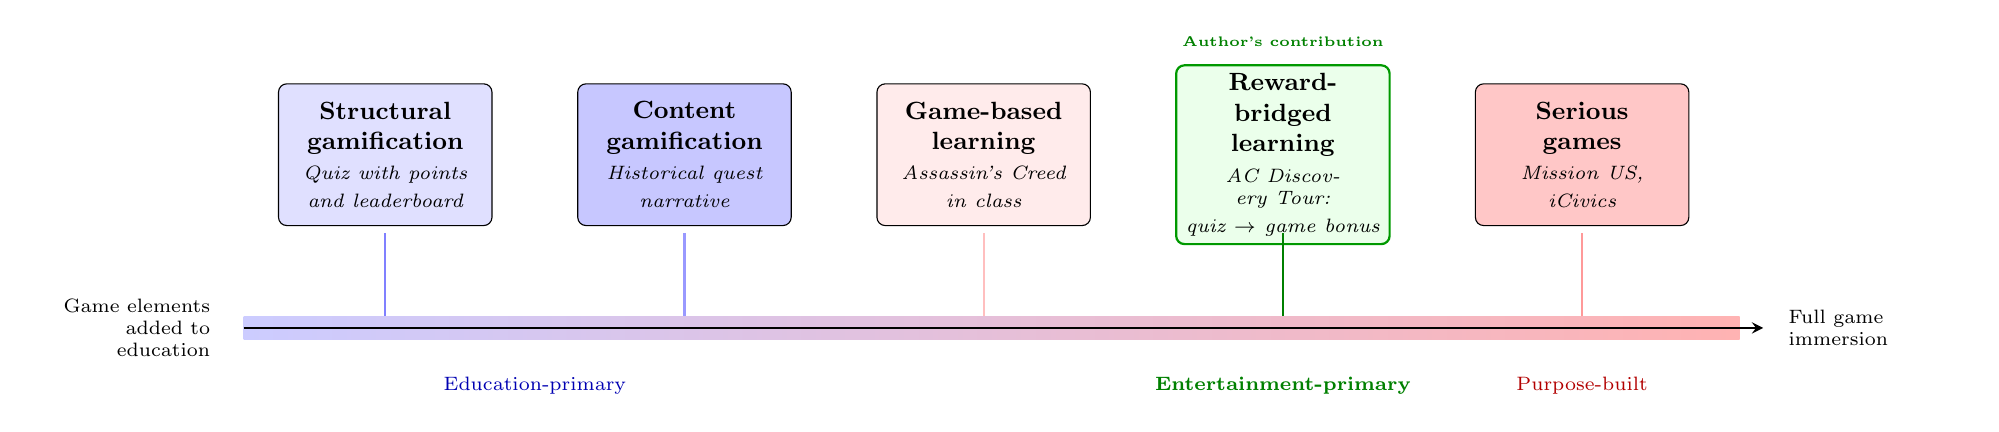
\begin{tikzpicture}[
  every node/.style={font=\small},
  levelbox/.style={rectangle, draw, rounded corners=3pt, minimum width=2.6cm,
    minimum height=1.8cm, text width=2.5cm, align=center, font=\small,
    inner sep=3pt},
  novelbox/.style={rectangle, draw, rounded corners=3pt, minimum width=2.6cm,
    minimum height=1.8cm, text width=2.5cm, align=center, font=\small,
    inner sep=3pt, thick, draw=green!60!black},
]

% Gradient arrow bar
\shade[left color=blue!20, right color=red!30] (0,-0.15) rectangle (19,0.15);
\draw[thick, ->, >=stealth] (0,0) -- (19.3,0);

% Left label
\node[font=\scriptsize, text width=2.2cm, align=right, anchor=east] at (-0.3,0)
  {Game elements\\added to\\education};
% Right label
\node[font=\scriptsize, text width=2.2cm, align=left, anchor=west] at (19.5,0)
  {Full game\\immersion};

% Level 1: Structural gamification
\node[levelbox, fill=blue!12] (L1) at (1.8, 2.2)
  {\textbf{Structural\\gamification}\\[3pt]
   \scriptsize\itshape Quiz with points\\[-1pt]\scriptsize\itshape and leaderboard};
\draw[thick, blue!50] (1.8, 1.2) -- (1.8, 0.15);

% Level 2: Content gamification
\node[levelbox, fill=blue!22] (L2) at (5.6, 2.2)
  {\textbf{Content\\gamification}\\[3pt]
   \scriptsize\itshape Historical quest\\[-1pt]\scriptsize\itshape narrative};
\draw[thick, blue!40] (5.6, 1.2) -- (5.6, 0.15);

% Level 3: Game-based learning
\node[levelbox, fill=red!8] (L3) at (9.4, 2.2)
  {\textbf{Game-based\\learning}\\[3pt]
   \scriptsize\itshape Assassin's Creed\\[-1pt]\scriptsize\itshape in class};
\draw[thick, red!25] (9.4, 1.2) -- (9.4, 0.15);

% Level 4: Reward-bridged learning (NEW — author's contribution)
\node[novelbox, fill=green!8] (L4) at (13.2, 2.2)
  {\textbf{Reward-bridged\\learning}\\[3pt]
   \scriptsize\itshape AC Discovery Tour:\\[-1pt]\scriptsize\itshape quiz $\to$ game bonus};
\draw[thick, green!50!black] (13.2, 1.2) -- (13.2, 0.15);

% Level 5: Serious games
\node[levelbox, fill=red!22] (L5) at (17.0, 2.2)
  {\textbf{Serious\\games}\\[3pt]
   \scriptsize\itshape Mission US,\\[-1pt]\scriptsize\itshape iCivics};
\draw[thick, red!40] (17.0, 1.2) -- (17.0, 0.15);

% Directionality annotation below
\node[font=\scriptsize, blue!70!black, anchor=north] at (3.7, -0.5)
  {Education-primary};
\node[font=\scriptsize, green!50!black, anchor=north, font=\scriptsize\bfseries] at (13.2, -0.5)
  {Entertainment-primary};
\node[font=\scriptsize, red!70!black, anchor=north] at (17.0, -0.5)
  {Purpose-built};

% Novel contribution marker
\node[font=\tiny\bfseries, green!50!black, anchor=south] at (13.2, 3.45)
  {Author's contribution};

\end{tikzpicture}
}
\caption{Conceptual spectrum of game integration in history education: from structural gamification to serious games. Reward-bridged learning (highlighted) is the author's proposed addition, occupying the position where education is integrated into entertainment games through incentive mechanisms (see Section~\ref{sec:gamification-review}).}
\label{fig:gamification-spectrum}
\end{figure}

\begin{figure}[!h]
\centering
\resizebox{\textwidth}{!}{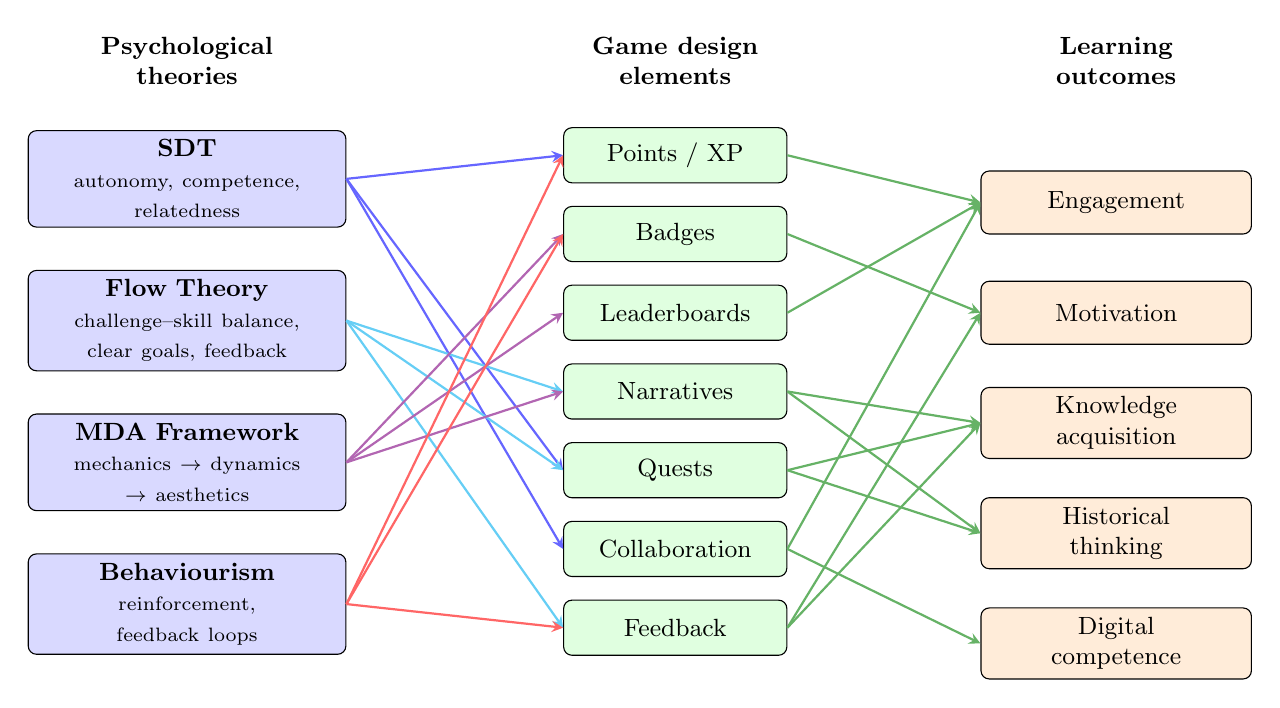
\begin{tikzpicture}[
  node distance=0.5cm,
  theorybox/.style={rectangle, draw, rounded corners=3pt, fill=#1!15,
    text width=3.8cm, minimum height=1cm, align=center, font=\small},
  theorybox/.default=blue,
  elembox/.style={rectangle, draw, rounded corners=3pt, fill=green!12,
    text width=2.6cm, minimum height=0.7cm, align=center, font=\small},
  outbox/.style={rectangle, draw, rounded corners=3pt, fill=orange!15,
    text width=3.2cm, minimum height=0.8cm, align=center, font=\small},
  colhead/.style={font=\bfseries\small, align=center},
  arr/.style={->, >=stealth, thick, #1!60},
  arr/.default=gray
]

% Column headers
\node[colhead] (h1) at (0, 0) {Psychological\\theories};
\node[colhead] (h2) at (6.2, 0) {Game design\\elements};
\node[colhead] (h3) at (11.8, 0) {Learning\\outcomes};

% Column 1: Theories
\node[theorybox=blue] (sdt) at (0, -1.5) {\textbf{SDT}\\{\scriptsize autonomy, competence,}\\{\scriptsize relatedness}};
\node[theorybox=blue] (flow) at (0, -3.3) {\textbf{Flow Theory}\\{\scriptsize challenge--skill balance,}\\{\scriptsize clear goals, feedback}};
\node[theorybox=blue] (mda) at (0, -5.1) {\textbf{MDA Framework}\\{\scriptsize mechanics $\to$ dynamics}\\{\scriptsize $\to$ aesthetics}};
\node[theorybox=blue] (behav) at (0, -6.9) {\textbf{Behaviourism}\\{\scriptsize reinforcement,}\\{\scriptsize feedback loops}};

% Column 2: Game elements
\node[elembox] (points) at (6.2, -1.2) {Points / XP};
\node[elembox] (badges) at (6.2, -2.2) {Badges};
\node[elembox] (leader) at (6.2, -3.2) {Leaderboards};
\node[elembox] (narr) at (6.2, -4.2) {Narratives};
\node[elembox] (quests) at (6.2, -5.2) {Quests};
\node[elembox] (collab) at (6.2, -6.2) {Collaboration};
\node[elembox] (feedb) at (6.2, -7.2) {Feedback};

% Column 3: Outcomes
\node[outbox] (engage) at (11.8, -1.8) {Engagement};
\node[outbox] (motiv) at (11.8, -3.2) {Motivation};
\node[outbox] (knowl) at (11.8, -4.6) {Knowledge\\acquisition};
\node[outbox] (hist) at (11.8, -6.0) {Historical\\thinking};
\node[outbox] (digcomp) at (11.8, -7.4) {Digital\\competence};

% Arrows: SDT → elements (competence, autonomy, relatedness)
\draw[arr=blue] (sdt.east) -- (points.west);
\draw[arr=blue] (sdt.east) -- (quests.west);
\draw[arr=blue] (sdt.east) -- (collab.west);

% Arrows: Flow → elements
\draw[arr=cyan] (flow.east) -- (narr.west);
\draw[arr=cyan] (flow.east) -- (quests.west);
\draw[arr=cyan] (flow.east) -- (feedb.west);

% Arrows: MDA → elements
\draw[arr=violet] (mda.east) -- (narr.west);
\draw[arr=violet] (mda.east) -- (badges.west);
\draw[arr=violet] (mda.east) -- (leader.west);

% Arrows: Behaviourism → elements
\draw[arr=red] (behav.east) -- (points.west);
\draw[arr=red] (behav.east) -- (badges.west);
\draw[arr=red] (behav.east) -- (feedb.west);

% Arrows: elements → outcomes
\draw[arr=green!50!black] (points.east) -- (engage.west);
\draw[arr=green!50!black] (badges.east) -- (motiv.west);
\draw[arr=green!50!black] (leader.east) -- (engage.west);
\draw[arr=green!50!black] (narr.east) -- (hist.west);
\draw[arr=green!50!black] (quests.east) -- (knowl.west);
\draw[arr=green!50!black] (collab.east) -- (digcomp.west);
\draw[arr=green!50!black] (feedb.east) -- (motiv.west);
\draw[arr=green!50!black] (narr.east) -- (knowl.west);
\draw[arr=green!50!black] (quests.east) -- (hist.west);
\draw[arr=green!50!black] (collab.east) -- (engage.west);
\draw[arr=green!50!black] (feedb.east) -- (knowl.west);

\end{tikzpicture}
}
\caption{Theoretical integration model: psychological foundations of gamification mechanisms and their expected learning outcomes (see Section~\ref{sec:gamification-review}).}
\label{fig:gamification-theory}
\end{figure}

\begin{figure}[!h]
\centering
\resizebox{\textwidth}{!}{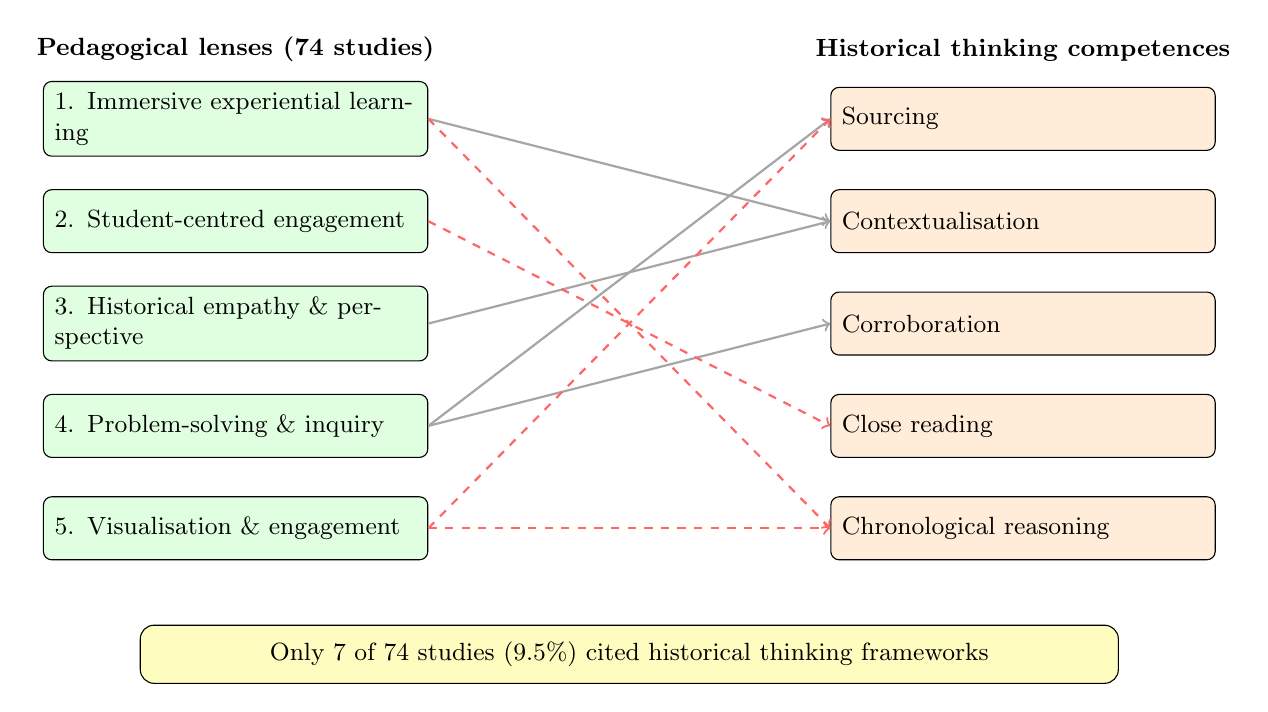
\begin{tikzpicture}[
  every node/.style={font=\small},
  pedbox/.style={rectangle, draw, rounded corners=3pt, fill=green!12,
    minimum width=4.8cm, minimum height=0.8cm, text width=4.6cm,
    align=left, font=\small, inner sep=4pt},
  histbox/.style={rectangle, draw, rounded corners=3pt, fill=orange!15,
    minimum width=4.8cm, minimum height=0.8cm, text width=4.6cm,
    align=left, font=\small, inner sep=4pt},
  colhead/.style={font=\small\bfseries, anchor=south},
  callout/.style={rectangle, draw, rounded corners=5pt, fill=yellow!25,
    font=\small, inner sep=6pt, text width=12cm, align=center},
]

% Column headers
\node[colhead] at (0, 0.6) {Pedagogical lenses (74 studies)};
\node[colhead] at (10, 0.6) {Historical thinking competences};

% Left column: Pedagogical lenses
\node[pedbox] (P1) at (0, 0) {1. Immersive experiential learning};
\node[pedbox] (P2) at (0, -1.3) {2. Student-centred engagement};
\node[pedbox] (P3) at (0, -2.6) {3. Historical empathy \& perspective};
\node[pedbox] (P4) at (0, -3.9) {4. Problem-solving \& inquiry};
\node[pedbox] (P5) at (0, -5.2) {5. Visualisation \& engagement};

% Right column: Wineburg's historical thinking
\node[histbox] (H1) at (10, 0) {Sourcing};
\node[histbox] (H2) at (10, -1.3) {Contextualisation};
\node[histbox] (H3) at (10, -2.6) {Corroboration};
\node[histbox] (H4) at (10, -3.9) {Close reading};
\node[histbox] (H5) at (10, -5.2) {Chronological reasoning};

% Solid arrows: established connections
\draw[->, thick, gray!70] (P1.east) -- (H2.west);
\draw[->, thick, gray!70] (P3.east) -- (H2.west);
\draw[->, thick, gray!70] (P4.east) -- (H1.west);
\draw[->, thick, gray!70] (P4.east) -- (H3.west);

% Dashed arrows: underexplored alignments
\draw[->, dashed, red!60, thick] (P1.east) -- (H5.west);
\draw[->, dashed, red!60, thick] (P2.east) -- (H4.west);
\draw[->, dashed, red!60, thick] (P5.east) -- (H1.west);
\draw[->, dashed, red!60, thick] (P5.east) -- (H5.west);

% Callout box
\node[callout] at (5, -6.8)
  {Only 7 of 74 studies (9.5\%) cited historical thinking frameworks};

\end{tikzpicture}
}
\caption{Mapping of pedagogical conceptualisations to core historical thinking competences: established connections (solid) and underexplored alignments (dashed) (see Section~\ref{sec:gamification-review}).}
\label{fig:pedagogical-disciplinary-gap}
\end{figure}

\begin{figure}[!h]
\centering
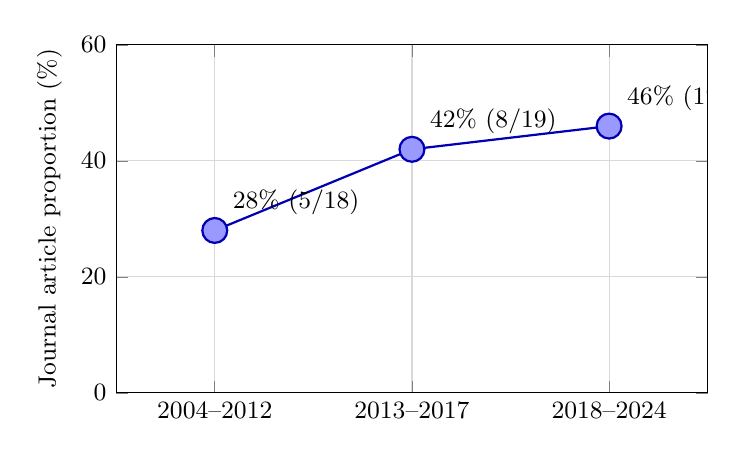
\begin{tikzpicture}
\begin{axis}[
    width=0.75\textwidth,
    height=6cm,
    ylabel={Journal article proportion (\%)},
    symbolic x coords={2004--2012, 2013--2017, 2018--2024},
    xtick=data,
    ymin=0, ymax=60,
    enlarge x limits=0.25,
    grid=major,
    grid style={gray!30},
    x tick label style={font=\small},
    y tick label style={font=\small},
    ylabel style={font=\small},
    mark size=3pt,
]

\addplot[thick, blue!70!black, mark=*, mark options={fill=blue!40, scale=1.5}]
    coordinates {
    (2004--2012, 28)
    (2013--2017, 42)
    (2018--2024, 46)
};

% Data labels with n values
\node[font=\small, anchor=south west, xshift=3pt, yshift=2pt]
    at (axis cs:2004--2012, 28) {28\% (5/18)};
\node[font=\small, anchor=south west, xshift=3pt, yshift=2pt]
    at (axis cs:2013--2017, 42) {42\% (8/19)};
\node[font=\small, anchor=south west, xshift=3pt, yshift=2pt]
    at (axis cs:2018--2024, 46) {46\% (17/37)};

\end{axis}
\end{tikzpicture}
\caption{Journal article proportion across three research periods, indicating gradual field maturation from conference-dominated to more journal-based dissemination (see Section~\ref{sec:evidence-base}).}
\label{fig:publication-type-evolution}
\end{figure}


\begin{figure}[htbp]
\centering
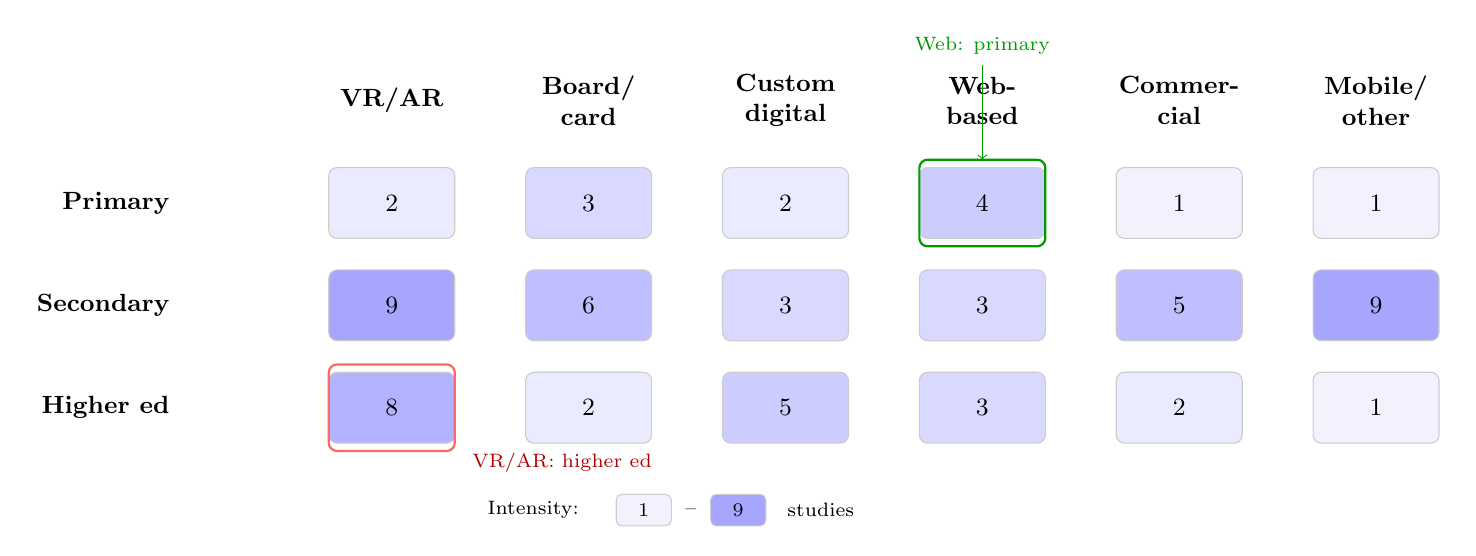
\begin{tikzpicture}[
    cell/.style={minimum width=1.6cm, minimum height=0.9cm, align=center, font=\small},
    hdr/.style={font=\small\bfseries, align=center, text width=1.6cm},
]

% Column spacing
\def\cs{2.5}  % column step

% Column headers
\node[hdr] at (0, 0) {};
\node[hdr] at (1*\cs, 0) {VR/AR};
\node[hdr] at (2*\cs, 0) {Board/\\card};
\node[hdr] at (3*\cs, 0) {Custom\\digital};
\node[hdr] at (4*\cs, 0) {Web-\\based};
\node[hdr] at (5*\cs, 0) {Commer-\\cial};
\node[hdr] at (6*\cs, 0) {Mobile/\\other};

% Row spacing
\def\rs{1.3}  % row step

% Row headers
\node[font=\small\bfseries, anchor=east] at (-0.2, -1*\rs) {Primary};
\node[font=\small\bfseries, anchor=east] at (-0.2, -2*\rs) {Secondary};
\node[font=\small\bfseries, anchor=east] at (-0.2, -3*\rs) {Higher ed};

% Primary row
\node[cell, fill=blue!8, draw=gray!40, rounded corners=3pt] at (1*\cs, -1*\rs) {2};
\node[cell, fill=blue!15, draw=gray!40, rounded corners=3pt] at (2*\cs, -1*\rs) {3};
\node[cell, fill=blue!8, draw=gray!40, rounded corners=3pt] at (3*\cs, -1*\rs) {2};
\node[cell, fill=blue!20, draw=gray!40, rounded corners=3pt] at (4*\cs, -1*\rs) {4};
\node[cell, fill=blue!5, draw=gray!40, rounded corners=3pt] at (5*\cs, -1*\rs) {1};
\node[cell, fill=blue!5, draw=gray!40, rounded corners=3pt] at (6*\cs, -1*\rs) {1};

% Secondary row
\node[cell, fill=blue!35, draw=gray!40, rounded corners=3pt] at (1*\cs, -2*\rs) {9};
\node[cell, fill=blue!25, draw=gray!40, rounded corners=3pt] at (2*\cs, -2*\rs) {6};
\node[cell, fill=blue!15, draw=gray!40, rounded corners=3pt] at (3*\cs, -2*\rs) {3};
\node[cell, fill=blue!15, draw=gray!40, rounded corners=3pt] at (4*\cs, -2*\rs) {3};
\node[cell, fill=blue!25, draw=gray!40, rounded corners=3pt] at (5*\cs, -2*\rs) {5};
\node[cell, fill=blue!35, draw=gray!40, rounded corners=3pt] at (6*\cs, -2*\rs) {9};

% Higher ed row
\node[cell, fill=blue!30, draw=gray!40, rounded corners=3pt] at (1*\cs, -3*\rs) {8};
\node[cell, fill=blue!8, draw=gray!40, rounded corners=3pt] at (2*\cs, -3*\rs) {2};
\node[cell, fill=blue!20, draw=gray!40, rounded corners=3pt] at (3*\cs, -3*\rs) {5};
\node[cell, fill=blue!15, draw=gray!40, rounded corners=3pt] at (4*\cs, -3*\rs) {3};
\node[cell, fill=blue!8, draw=gray!40, rounded corners=3pt] at (5*\cs, -3*\rs) {2};
\node[cell, fill=blue!5, draw=gray!40, rounded corners=3pt] at (6*\cs, -3*\rs) {1};

% Highlight annotations (outside the grid)
\draw[red!60, thick, rounded corners=3pt]
    (1*\cs-0.8, -3*\rs-0.55) rectangle (1*\cs+0.8, -3*\rs+0.55);
\node[font=\scriptsize, text=red!70!black, anchor=west] at (1*\cs+0.9, -3*\rs-0.7) {VR/AR: higher ed};

\draw[green!60!black, thick, rounded corners=3pt]
    (4*\cs-0.8, -1*\rs-0.55) rectangle (4*\cs+0.8, -1*\rs+0.55);
\node[font=\scriptsize, text=green!60!black] at (4*\cs, 0.7) {Web: primary};
\draw[green!60!black, thin, ->] (4*\cs, 0.45) -- (4*\cs, -1*\rs+0.55);

% Color scale legend (bottom, well separated)
\node[font=\scriptsize, anchor=east] at (2*\cs, -3*\rs - 1.3) {Intensity:};
\node[cell, fill=blue!5, draw=gray!40, rounded corners=2pt, minimum width=0.7cm, minimum height=0.4cm, font=\scriptsize] at (2*\cs+0.7, -3*\rs - 1.3) {1};
\node[font=\scriptsize] at (2*\cs+1.3, -3*\rs - 1.3) {--};
\node[cell, fill=blue!35, draw=gray!40, rounded corners=2pt, minimum width=0.7cm, minimum height=0.4cm, font=\scriptsize] at (2*\cs+1.9, -3*\rs - 1.3) {9};
\node[font=\scriptsize, anchor=west] at (2*\cs+2.4, -3*\rs - 1.3) {studies};

\end{tikzpicture}
\caption{Cross-tabulation of education level and game type across 74 studies: cell values indicate study counts, colour intensity reflects density (some studies span multiple categories)}
\label{fig:evidence-cross-dimensions}
\end{figure}


\begin{figure}[!h]
\centering
\resizebox{\textwidth}{!}{%
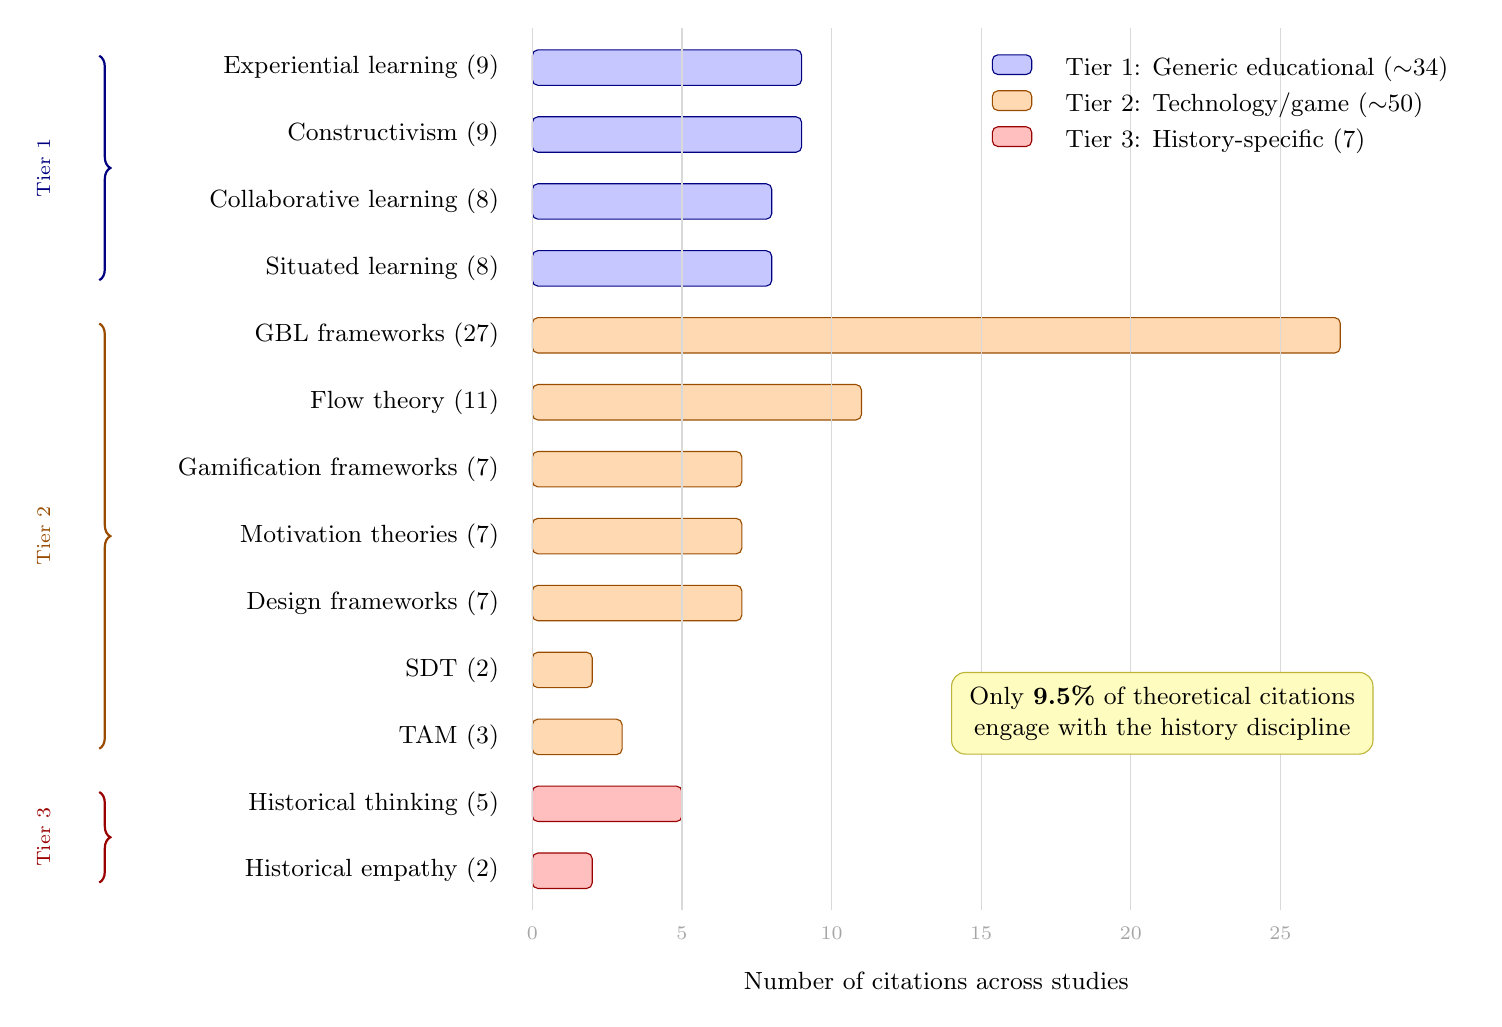
\begin{tikzpicture}

% Bar dimensions
\def\barheight{0.45}
\def\yscale{0.85}
\def\xscale{0.38}

% Tier labels (right-aligned y-axis labels)
\foreach \y/\label in {
    0/{Historical empathy (2)},
    1/{Historical thinking (5)},
    2/{TAM (3)},
    3/{SDT (2)},
    4/{Design frameworks (7)},
    5/{Motivation theories (7)},
    6/{Gamification frameworks (7)},
    7/{Flow theory (11)},
    8/{GBL frameworks (27)},
    9/{Situated learning (8)},
    10/{Collaborative learning (8)},
    11/{Constructivism (9)},
    12/{Experiential learning (9)}
} {
    \node[font=\small, anchor=east] at (-0.3, \y*\yscale) {\label};
}

% Tier 3 — History-discipline-specific (red)
\fill[red!25, draw=red!60!black, rounded corners=2pt] (0, 0*\yscale-\barheight/2) rectangle (2*\xscale, 0*\yscale+\barheight/2);
\fill[red!25, draw=red!60!black, rounded corners=2pt] (0, 1*\yscale-\barheight/2) rectangle (5*\xscale, 1*\yscale+\barheight/2);

% Tier 2 — Technology/game-specific (orange)
\fill[orange!30, draw=orange!60!black, rounded corners=2pt] (0, 2*\yscale-\barheight/2) rectangle (3*\xscale, 2*\yscale+\barheight/2);
\fill[orange!30, draw=orange!60!black, rounded corners=2pt] (0, 3*\yscale-\barheight/2) rectangle (2*\xscale, 3*\yscale+\barheight/2);
\fill[orange!30, draw=orange!60!black, rounded corners=2pt] (0, 4*\yscale-\barheight/2) rectangle (7*\xscale, 4*\yscale+\barheight/2);
\fill[orange!30, draw=orange!60!black, rounded corners=2pt] (0, 5*\yscale-\barheight/2) rectangle (7*\xscale, 5*\yscale+\barheight/2);
\fill[orange!30, draw=orange!60!black, rounded corners=2pt] (0, 6*\yscale-\barheight/2) rectangle (7*\xscale, 6*\yscale+\barheight/2);
\fill[orange!30, draw=orange!60!black, rounded corners=2pt] (0, 7*\yscale-\barheight/2) rectangle (11*\xscale, 7*\yscale+\barheight/2);
\fill[orange!30, draw=orange!60!black, rounded corners=2pt] (0, 8*\yscale-\barheight/2) rectangle (27*\xscale, 8*\yscale+\barheight/2);

% Tier 1 — Generic educational (blue)
\fill[blue!22, draw=blue!50!black, rounded corners=2pt] (0, 9*\yscale-\barheight/2) rectangle (8*\xscale, 9*\yscale+\barheight/2);
\fill[blue!22, draw=blue!50!black, rounded corners=2pt] (0, 10*\yscale-\barheight/2) rectangle (8*\xscale, 10*\yscale+\barheight/2);
\fill[blue!22, draw=blue!50!black, rounded corners=2pt] (0, 11*\yscale-\barheight/2) rectangle (9*\xscale, 11*\yscale+\barheight/2);
\fill[blue!22, draw=blue!50!black, rounded corners=2pt] (0, 12*\yscale-\barheight/2) rectangle (9*\xscale, 12*\yscale+\barheight/2);

% X-axis
\draw[gray!50] (0, -0.5) -- (0, 12*\yscale+0.5);
\foreach \x in {0, 5, 10, 15, 20, 25} {
    \draw[gray!30] (\x*\xscale, -0.5) -- (\x*\xscale, 12*\yscale+0.5);
    \node[font=\scriptsize, text=gray!70] at (\x*\xscale, -0.8) {\x};
}
\node[font=\small] at (13.5*\xscale, -1.4) {Number of citations across studies};

% Tier bracket labels
\draw[decorate, decoration={brace, amplitude=4pt, mirror}, red!60!black, thick]
    (-5.5, -0.15) -- (-5.5, 1*\yscale+0.15);
\node[font=\scriptsize, text=red!60!black, rotate=90, anchor=south] at (-6.0, 0.5*\yscale) {Tier 3};

\draw[decorate, decoration={brace, amplitude=4pt, mirror}, orange!60!black, thick]
    (-5.5, 2*\yscale-0.15) -- (-5.5, 8*\yscale+0.15);
\node[font=\scriptsize, text=orange!60!black, rotate=90, anchor=south] at (-6.0, 5*\yscale) {Tier 2};

\draw[decorate, decoration={brace, amplitude=4pt, mirror}, blue!50!black, thick]
    (-5.5, 9*\yscale-0.15) -- (-5.5, 12*\yscale+0.15);
\node[font=\scriptsize, text=blue!50!black, rotate=90, anchor=south] at (-6.0, 10.5*\yscale) {Tier 1};

% Callout box
\node[draw=yellow!70!black, fill=yellow!25, rounded corners=5pt,
      text width=5cm, align=center, font=\small,
      inner sep=5pt] at (8.0, 2.0)
    {Only \textbf{9.5\%} of theoretical citations\\engage with the history discipline};

% Legend
\node[anchor=north west, font=\small] at (5.5, 12*\yscale+0.3) {
    \begin{tabular}{ll}
    \tikz\fill[blue!22, draw=blue!50!black, rounded corners=2pt] (0,0) rectangle (0.5,0.25); & Tier~1: Generic educational (${\sim}$34) \\[2pt]
    \tikz\fill[orange!30, draw=orange!60!black, rounded corners=2pt] (0,0) rectangle (0.5,0.25); & Tier~2: Technology/game (${\sim}$50) \\[2pt]
    \tikz\fill[red!25, draw=red!60!black, rounded corners=2pt] (0,0) rectangle (0.5,0.25); & Tier~3: History-specific (7) \\
    \end{tabular}
};

\end{tikzpicture}%
}%
\caption{Three-tier classification of theoretical frameworks cited across 74 studies: generic educational theories (Tier~1, $\sim$34 citations), technology and game-specific frameworks (Tier~2, $\sim$50 citations), and history-discipline-specific frameworks (Tier~3, only 7 citations) (see Section~\ref{sec:evidence-base}).}
\label{fig:theoretical-framework-tiers}
\end{figure}


% --- Chapter 1 Section 1.4 (DigComp) supplementary figures ---

\begin{figure}[!h]
\centering
\resizebox{\textwidth}{!}{%
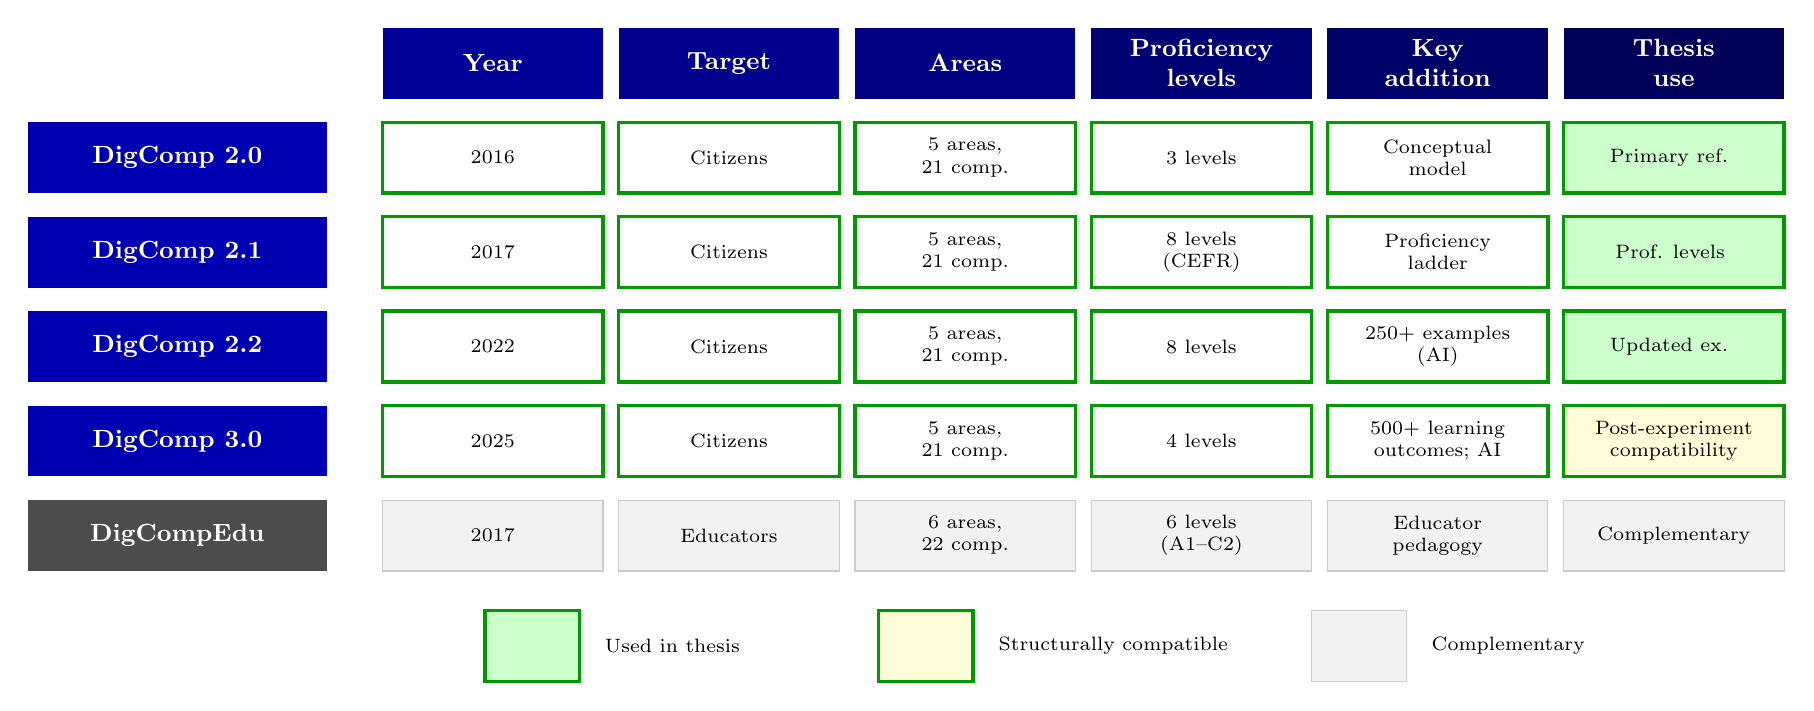
\begin{tikzpicture}[
  hdr/.style={font=\small\bfseries, text=white, minimum height=0.9cm,
    minimum width=2.8cm, align=center},
  rhdr/.style={font=\small\bfseries, text=white, minimum height=0.9cm,
    minimum width=3.8cm, align=center, anchor=east},
  cell/.style={rectangle, draw=gray!40, minimum height=0.9cm,
    minimum width=2.8cm, align=center, font=\scriptsize},
  usedcell/.style={cell, draw=green!60!black, line width=1.2pt},
  graycell/.style={cell, fill=gray!10},
  usedr/.style={font=\small\bfseries, text=white, minimum height=0.9cm,
    minimum width=3.8cm, align=center, anchor=east, fill=blue!70!black},
  grayr/.style={font=\small\bfseries, text=white, minimum height=0.9cm,
    minimum width=3.8cm, align=center, anchor=east, fill=gray!60!black},
]

% Column spacing
\def\colw{3.0}

% Column headers
\node[hdr, fill=blue!60!black] at (0, 0) {Year};
\node[hdr, fill=blue!55!black] at (\colw, 0) {Target};
\node[hdr, fill=blue!50!black] at (2*\colw, 0) {Areas};
\node[hdr, fill=blue!45!black] at (3*\colw, 0) {Proficiency\\levels};
\node[hdr, fill=blue!40!black] at (4*\colw, 0) {Key\\addition};
\node[hdr, fill=blue!35!black] at (5*\colw, 0) {Thesis\\use};

% Row 1: DigComp 2.0 — used in thesis (green border)
\node[usedr] at (-2.1, -1.2) {DigComp 2.0};
\node[usedcell] at (0, -1.2) {2016};
\node[usedcell] at (\colw, -1.2) {Citizens};
\node[usedcell] at (2*\colw, -1.2) {5 areas,\\21 comp.};
\node[usedcell] at (3*\colw, -1.2) {3 levels};
\node[usedcell] at (4*\colw, -1.2) {Conceptual\\model};
\node[usedcell, fill=green!20] at (5*\colw, -1.2) {Primary ref. \checkmark};

% Row 2: DigComp 2.1 — used in thesis (green border)
\node[usedr] at (-2.1, -2.4) {DigComp 2.1};
\node[usedcell] at (0, -2.4) {2017};
\node[usedcell] at (\colw, -2.4) {Citizens};
\node[usedcell] at (2*\colw, -2.4) {5 areas,\\21 comp.};
\node[usedcell] at (3*\colw, -2.4) {8 levels\\(CEFR)};
\node[usedcell] at (4*\colw, -2.4) {Proficiency\\ladder};
\node[usedcell, fill=green!20] at (5*\colw, -2.4) {Prof. levels \checkmark};

% Row 3: DigComp 2.2 — used in thesis (green border)
\node[usedr] at (-2.1, -3.6) {DigComp 2.2};
\node[usedcell] at (0, -3.6) {2022};
\node[usedcell] at (\colw, -3.6) {Citizens};
\node[usedcell] at (2*\colw, -3.6) {5 areas,\\21 comp.};
\node[usedcell] at (3*\colw, -3.6) {8 levels};
\node[usedcell] at (4*\colw, -3.6) {250+ examples\\(AI)};
\node[usedcell, fill=green!20] at (5*\colw, -3.6) {Updated ex. \checkmark};

% Row 4: DigComp 3.0 — contextual (green border, published after experiment)
\node[usedr] at (-2.1, -4.8) {DigComp 3.0};
\node[usedcell] at (0, -4.8) {2025};
\node[usedcell] at (\colw, -4.8) {Citizens};
\node[usedcell] at (2*\colw, -4.8) {5 areas,\\21 comp.};
\node[usedcell] at (3*\colw, -4.8) {4 levels};
\node[usedcell] at (4*\colw, -4.8) {500+ learning\\outcomes; AI};
\node[usedcell, fill=yellow!15] at (5*\colw, -4.8) {Post-experiment\\compatibility};

% Row 5: DigCompEdu — complementary (gray)
\node[grayr] at (-2.1, -6.0) {DigCompEdu};
\node[graycell] at (0, -6.0) {2017};
\node[graycell] at (\colw, -6.0) {Educators};
\node[graycell] at (2*\colw, -6.0) {6 areas,\\22 comp.};
\node[graycell] at (3*\colw, -6.0) {6 levels\\(A1--C2)};
\node[graycell] at (4*\colw, -6.0) {Educator\\pedagogy};
\node[graycell] at (5*\colw, -6.0) {Complementary};

% Legend
\node[usedcell, fill=green!20, minimum width=1.2cm] at (0.5, -7.4) {};
\node[font=\scriptsize, anchor=west] at (1.3, -7.4) {Used in thesis};
\node[usedcell, fill=yellow!15, minimum width=1.2cm] at (5.5, -7.4) {};
\node[font=\scriptsize, anchor=west] at (6.3, -7.4) {Structurally compatible};
\node[graycell, minimum width=1.2cm] at (11.0, -7.4) {};
\node[font=\scriptsize, anchor=west] at (11.8, -7.4) {Complementary};

\end{tikzpicture}%
}% end resizebox
\caption{The DigComp framework family: evolution and application in this thesis. All DigComp versions maintain the same five-area, 21-competence structure; differences lie in proficiency granularity, illustrative examples, and --- in DigComp~3.0 --- learning outcomes and AI integration. DigCompEdu addresses educator-specific competences and is used as a complementary reference. This thesis uses DigComp~2.0 as the primary conceptual framework (consistent with \citeauthor{Titova2025cte}~\cite{Titova2025cte}), with proficiency levels from DigComp~2.1 and updated examples from DigComp~2.2. DigComp~3.0 \citep{Cosgrove2025}, published after the experimental study, is structurally compatible with the thesis findings (see Section~\ref{sec:digcomp}).}
\label{fig:digcomp-framework-landscape}
\end{figure}


\begin{figure}[!h]
\centering
\resizebox{\textwidth}{!}{%
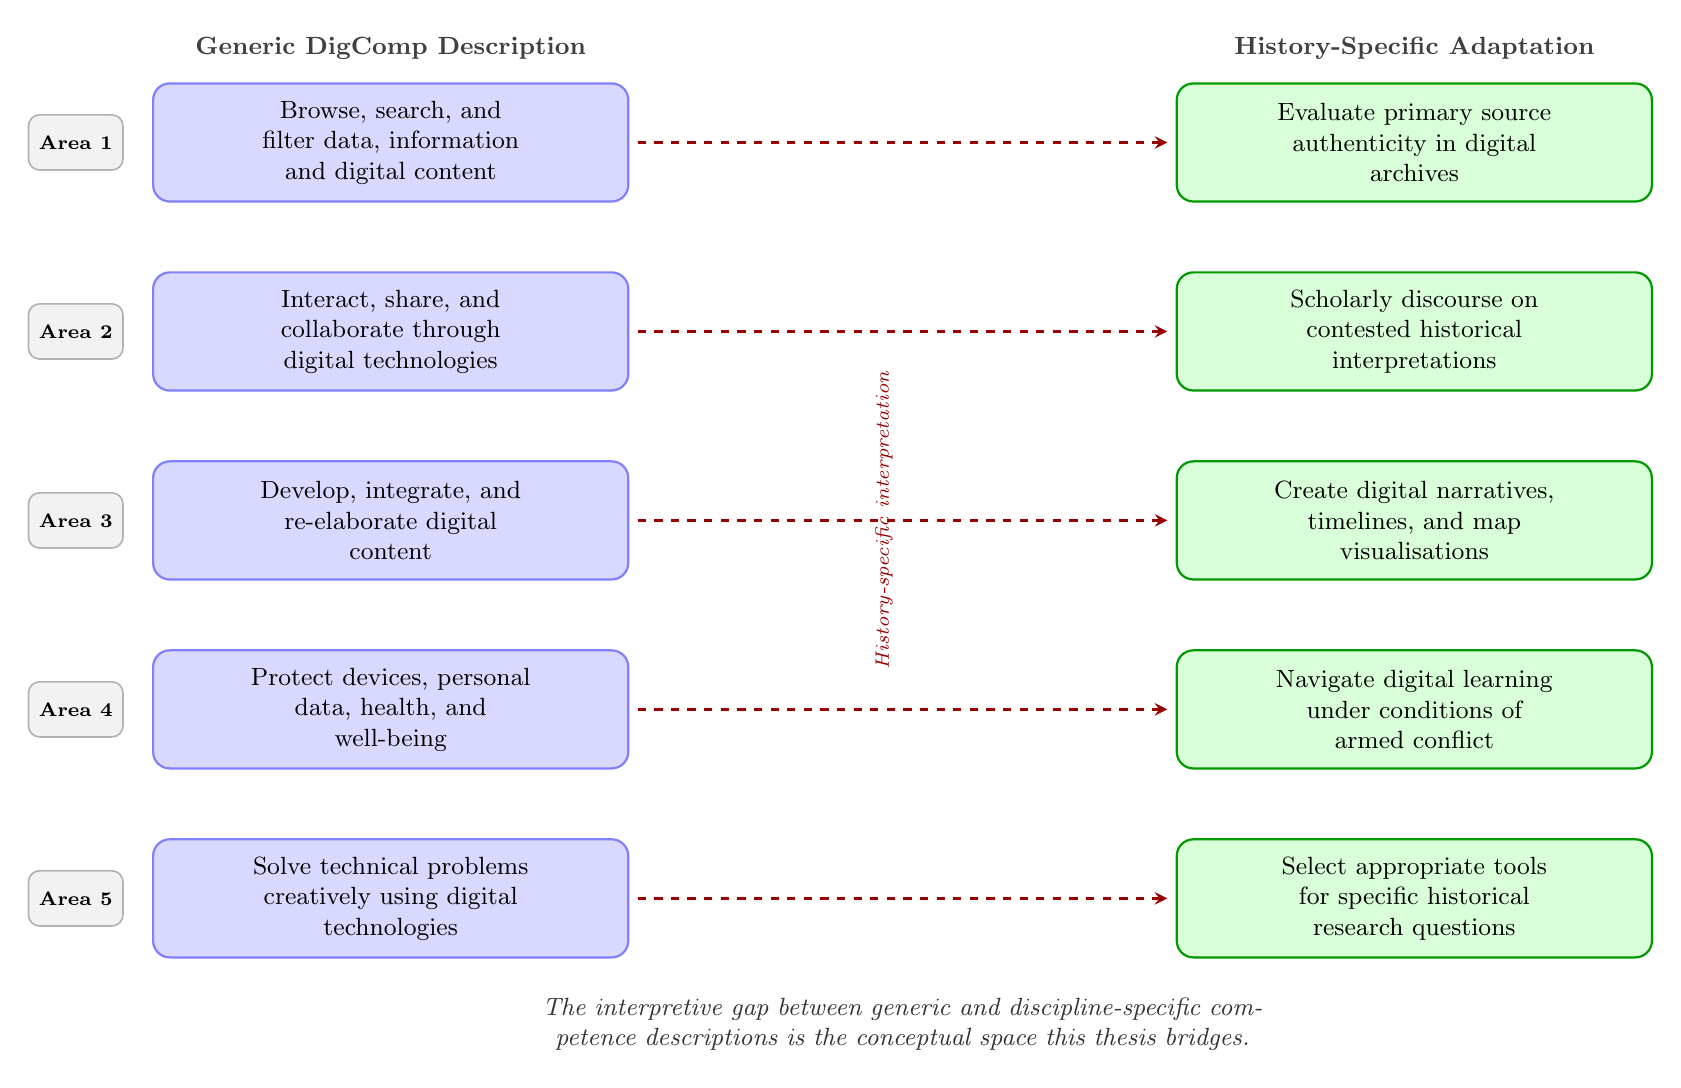
\begin{tikzpicture}[
  % Column styles
  generic/.style={rectangle, rounded corners=6pt, draw=blue!50, fill=blue!15,
    text width=5.8cm, minimum height=1.5cm, align=center, font=\small,
    line width=0.8pt},
  adapted/.style={rectangle, rounded corners=6pt, draw=green!60!black, fill=green!15,
    text width=5.8cm, minimum height=1.5cm, align=center, font=\small,
    line width=0.8pt},
  arealbl/.style={rectangle, rounded corners=4pt, draw=gray!60, fill=gray!10,
    minimum width=1.2cm, minimum height=0.7cm, align=center,
    font=\scriptsize\bfseries, line width=0.6pt},
  % Arrow style
  interp/.style={->, >=stealth, thick, draw=red!60!black, dashed, line width=1pt},
  % Annotation style
  note/.style={font=\small\itshape, text=gray!40!black, text width=14cm, align=center},
  % Header style
  header/.style={font=\small\bfseries\scshape, text=gray!50!black},
]

% Vertical spacing
\def\rowsep{2.4}
% Horizontal positions
\def\leftcol{-6.5}
\def\rightcol{6.5}
\def\arrowstart{-3.0}
\def\arrowend{3.0}
\def\arealblx{-10.5}

% Column headers
\node[header] at (\leftcol, 1.2) {Generic DigComp Description};
\node[header] at (0, 1.2) {};
\node[header] at (\rightcol, 1.2) {History-Specific Adaptation};

% --- Row 1: Information and data literacy ---
\node[arealbl] (a1) at (\arealblx, 0) {Area 1};
\node[generic] (g1) at (\leftcol, 0)
  {Browse, search, and\\filter data, information\\and digital content};
\node[adapted] (h1) at (\rightcol, 0)
  {Evaluate primary source\\authenticity in digital\\archives};
\draw[interp] ([xshift=3pt]g1.east) -- ([xshift=-3pt]h1.west);

% --- Row 2: Communication and collaboration ---
\node[arealbl] (a2) at (\arealblx, -\rowsep) {Area 2};
\node[generic] (g2) at (\leftcol, -\rowsep)
  {Interact, share, and\\collaborate through\\digital technologies};
\node[adapted] (h2) at (\rightcol, -\rowsep)
  {Scholarly discourse on\\contested historical\\interpretations};
\draw[interp] ([xshift=3pt]g2.east) -- ([xshift=-3pt]h2.west);

% --- Row 3: Digital content creation ---
\node[arealbl] (a3) at (\arealblx, -2*\rowsep) {Area 3};
\node[generic] (g3) at (\leftcol, -2*\rowsep)
  {Develop, integrate, and\\re-elaborate digital\\content};
\node[adapted] (h3) at (\rightcol, -2*\rowsep)
  {Create digital narratives,\\timelines, and map\\visualisations};
\draw[interp] ([xshift=3pt]g3.east) -- ([xshift=-3pt]h3.west);

% --- Row 4: Safety ---
\node[arealbl] (a4) at (\arealblx, -3*\rowsep) {Area 4};
\node[generic] (g4) at (\leftcol, -3*\rowsep)
  {Protect devices, personal\\data, health, and\\well-being};
\node[adapted] (h4) at (\rightcol, -3*\rowsep)
  {Navigate digital learning\\under conditions of\\armed conflict};
\draw[interp] ([xshift=3pt]g4.east) -- ([xshift=-3pt]h4.west);

% --- Row 5: Problem solving ---
\node[arealbl] (a5) at (\arealblx, -4*\rowsep) {Area 5};
\node[generic] (g5) at (\leftcol, -4*\rowsep)
  {Solve technical problems\\creatively using digital\\technologies};
\node[adapted] (h5) at (\rightcol, -4*\rowsep)
  {Select appropriate tools\\for specific historical\\research questions};
\draw[interp] ([xshift=3pt]g5.east) -- ([xshift=-3pt]h5.west);

% Central arrow label (placed once, vertically centred)
\node[font=\scriptsize\itshape, text=red!60!black, rotate=90, anchor=south]
  at (0, -2*\rowsep) {History-specific interpretation};

% Bottom annotation
\node[note] at (0, -4*\rowsep - 1.6)
  {The interpretive gap between generic and discipline-specific competence
   descriptions is the conceptual space this thesis bridges.};

\end{tikzpicture}%
}% end resizebox
\caption{History-specific interpretation of DigComp competence areas. Left: generic
descriptions from DigComp~2.0 \citep{Vuorikari2016}. Right: discipline-specific
adaptations developed in this thesis, grounded in the epistemological requirements
of historical inquiry \citep{Crymble2021, MonteSano2012} and the wartime
educational context \citep{UNESCO2023}. No existing literature provides such an
adaptation; this represents a contribution of the present study (see Section~\ref{sec:digcomp}).}
\label{fig:digcomp-history-adaptation}
\end{figure}


% --- Chapter 1 Section 1.3 (MRQS) supplementary figures ---

\begin{figure}[!h]
\centering
\resizebox{\textwidth}{!}{%
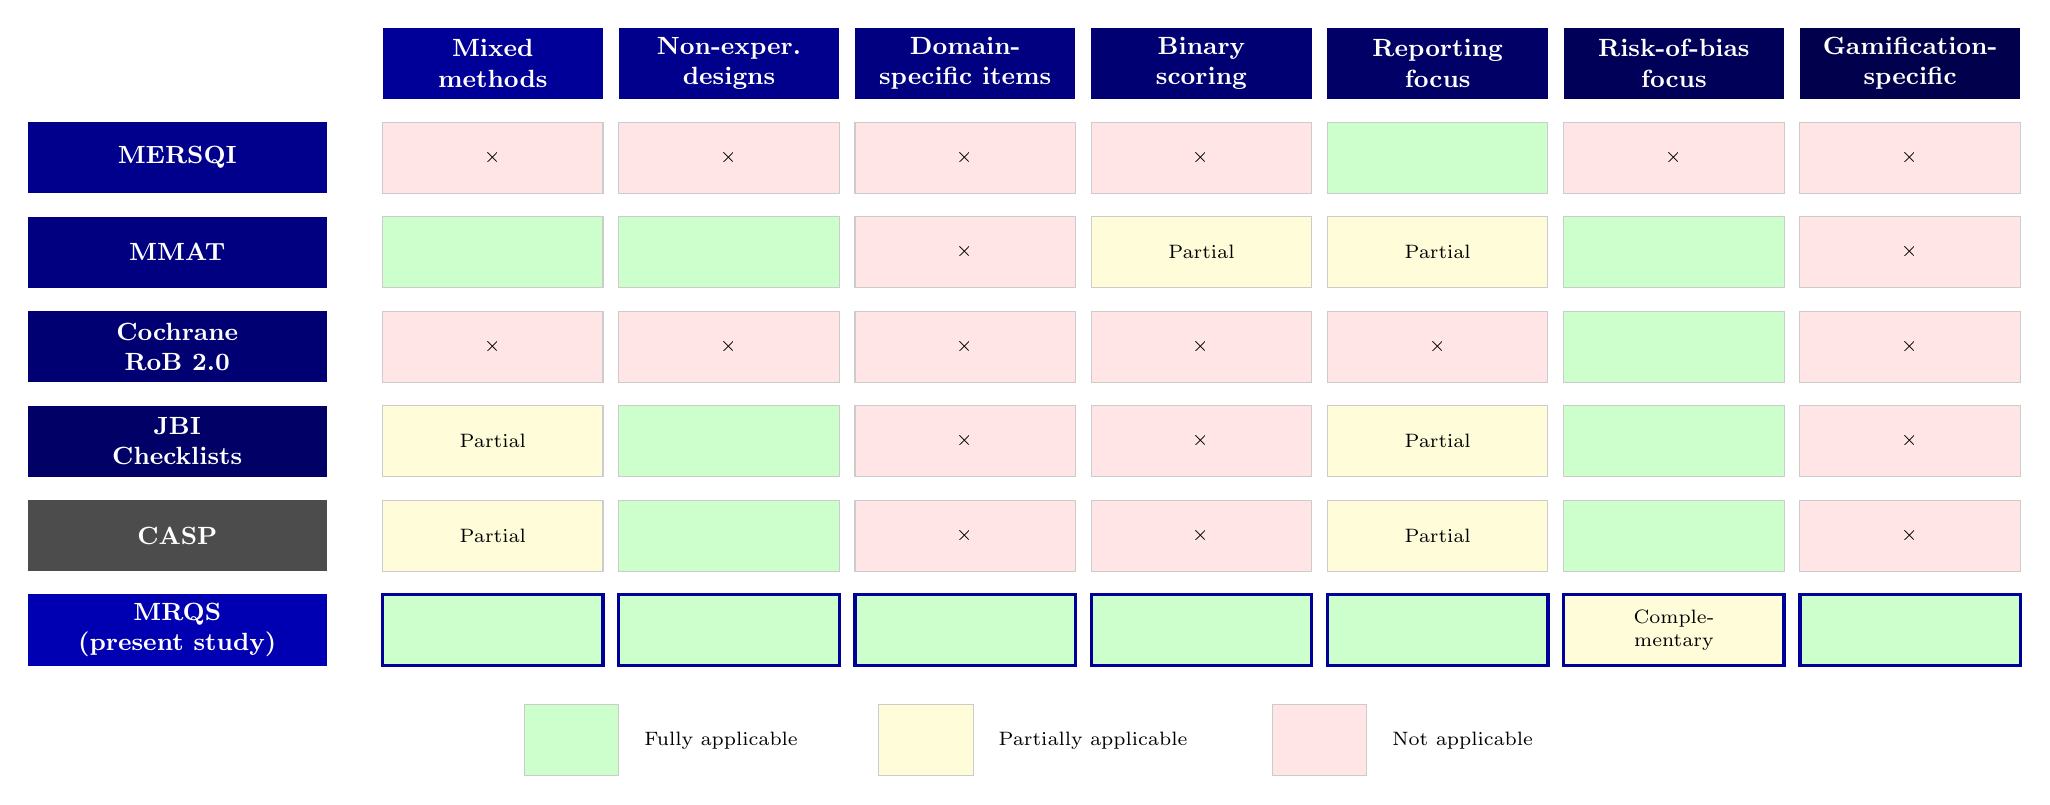
\begin{tikzpicture}[
  hdr/.style={font=\small\bfseries, text=white, minimum height=0.9cm,
    minimum width=2.8cm, align=center},
  rhdr/.style={font=\small\bfseries, text=white, minimum height=0.9cm,
    minimum width=3.8cm, align=center, anchor=east},
  cell/.style={rectangle, draw=gray!40, minimum height=0.9cm,
    minimum width=2.8cm, align=center, font=\scriptsize},
  strong/.style={cell, fill=green!20},
  moderate/.style={cell, fill=yellow!15},
  weak/.style={cell, fill=red!10},
  highlight/.style={cell, fill=green!20, draw=blue!60!black, line width=1.2pt},
  highlightr/.style={font=\small\bfseries, text=white, minimum height=0.9cm,
    minimum width=3.8cm, align=center, anchor=east, fill=blue!70!black},
]

% Column spacing
\def\colw{3.0}

% Column headers
\node[hdr, fill=blue!60!black] at (0, 0) {Mixed\\methods};
\node[hdr, fill=blue!55!black] at (\colw, 0) {Non-exper.\\designs};
\node[hdr, fill=blue!50!black] at (2*\colw, 0) {Domain-\\specific items};
\node[hdr, fill=blue!45!black] at (3*\colw, 0) {Binary\\scoring};
\node[hdr, fill=blue!40!black] at (4*\colw, 0) {Reporting\\focus};
\node[hdr, fill=blue!35!black] at (5*\colw, 0) {Risk-of-bias\\focus};
\node[hdr, fill=blue!30!black] at (6*\colw, 0) {Gamification-\\specific};

% Row 1: MERSQI
\node[rhdr, fill=blue!55!black] at (-2.1, -1.2) {MERSQI};
\node[weak] at (0, -1.2) {\texttimes};
\node[weak] at (\colw, -1.2) {\texttimes};
\node[weak] at (2*\colw, -1.2) {\texttimes};
\node[weak] at (3*\colw, -1.2) {\texttimes};
\node[strong] at (4*\colw, -1.2) {\checkmark};
\node[weak] at (5*\colw, -1.2) {\texttimes};
\node[weak] at (6*\colw, -1.2) {\texttimes};

% Row 2: MMAT
\node[rhdr, fill=blue!50!black] at (-2.1, -2.4) {MMAT};
\node[strong] at (0, -2.4) {\checkmark};
\node[strong] at (\colw, -2.4) {\checkmark};
\node[weak] at (2*\colw, -2.4) {\texttimes};
\node[moderate] at (3*\colw, -2.4) {Partial};
\node[moderate] at (4*\colw, -2.4) {Partial};
\node[strong] at (5*\colw, -2.4) {\checkmark};
\node[weak] at (6*\colw, -2.4) {\texttimes};

% Row 3: Cochrane RoB 2.0
\node[rhdr, fill=blue!45!black] at (-2.1, -3.6) {Cochrane\\RoB 2.0};
\node[weak] at (0, -3.6) {\texttimes};
\node[weak] at (\colw, -3.6) {\texttimes};
\node[weak] at (2*\colw, -3.6) {\texttimes};
\node[weak] at (3*\colw, -3.6) {\texttimes};
\node[weak] at (4*\colw, -3.6) {\texttimes};
\node[strong] at (5*\colw, -3.6) {\checkmark};
\node[weak] at (6*\colw, -3.6) {\texttimes};

% Row 4: JBI Checklists
\node[rhdr, fill=blue!40!black] at (-2.1, -4.8) {JBI\\Checklists};
\node[moderate] at (0, -4.8) {Partial};
\node[strong] at (\colw, -4.8) {\checkmark};
\node[weak] at (2*\colw, -4.8) {\texttimes};
\node[weak] at (3*\colw, -4.8) {\texttimes};
\node[moderate] at (4*\colw, -4.8) {Partial};
\node[strong] at (5*\colw, -4.8) {\checkmark};
\node[weak] at (6*\colw, -4.8) {\texttimes};

% Row 5: CASP
\node[rhdr, fill=gray!60!black] at (-2.1, -6.0) {CASP};
\node[moderate] at (0, -6.0) {Partial};
\node[strong] at (\colw, -6.0) {\checkmark};
\node[weak] at (2*\colw, -6.0) {\texttimes};
\node[weak] at (3*\colw, -6.0) {\texttimes};
\node[moderate] at (4*\colw, -6.0) {Partial};
\node[strong] at (5*\colw, -6.0) {\checkmark};
\node[weak] at (6*\colw, -6.0) {\texttimes};

% Row 6: MRQS (present study) — highlighted
\node[highlightr] at (-2.1, -7.2) {MRQS\\(present study)};
\node[highlight] at (0, -7.2) {\checkmark};
\node[highlight] at (\colw, -7.2) {\checkmark};
\node[highlight] at (2*\colw, -7.2) {\checkmark};
\node[highlight] at (3*\colw, -7.2) {\checkmark};
\node[highlight] at (4*\colw, -7.2) {\checkmark};
\node[moderate, draw=blue!60!black, line width=1.2pt] at (5*\colw, -7.2) {Comple-\\mentary};
\node[highlight] at (6*\colw, -7.2) {\checkmark};

% Legend
\node[strong, minimum width=1.2cm] at (1.0, -8.6) {};
\node[font=\scriptsize, anchor=west] at (1.8, -8.6) {Fully applicable};
\node[moderate, minimum width=1.2cm] at (5.5, -8.6) {};
\node[font=\scriptsize, anchor=west] at (6.3, -8.6) {Partially applicable};
\node[weak, minimum width=1.2cm] at (10.5, -8.6) {};
\node[font=\scriptsize, anchor=west] at (11.3, -8.6) {Not applicable};

\end{tikzpicture}%
}% end resizebox
\caption{Applicability of quality assessment tools to gamification research in history education. The MRQS (highlighted), developed for the present study, is the only instrument that simultaneously handles mixed-methods designs, includes domain-specific items, and uses binary scoring for reliability. Risk-of-bias assessment is addressed through a complementary adapted ROBIS instrument (see Section~\ref{sec:mrqs}).}
\label{fig:quality-tool-comparison}
\end{figure}


\begin{figure}[htbp]
\centering
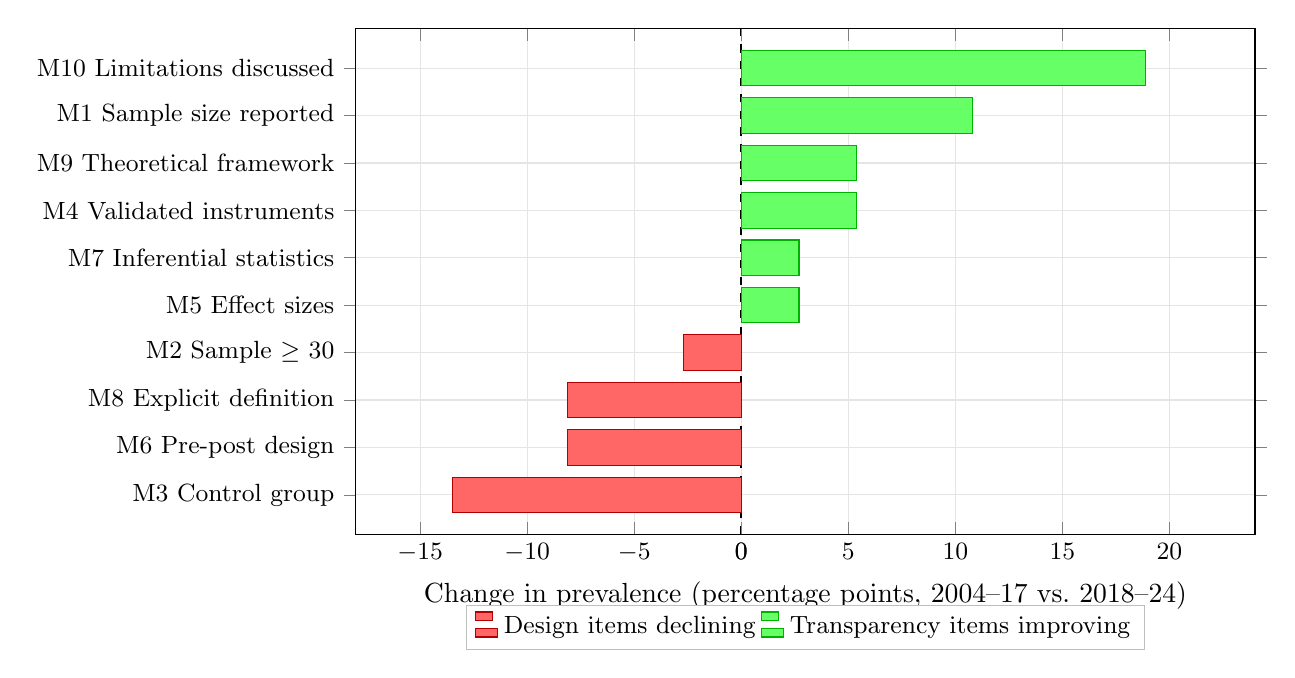
\begin{tikzpicture}
\begin{axis}[
    xbar,
    width=13cm,
    height=8cm,
    xlabel={Change in prevalence (percentage points, 2004--17 vs.\ 2018--24)},
    xmin=-18, xmax=24,
    ytick={0,1,2,3,4,5,6,7,8,9},
    yticklabels={
        {M3 Control group},
        {M6 Pre-post design},
        {M8 Explicit definition},
        {M2 Sample $\geq$ 30},
        {M5 Effect sizes},
        {M7 Inferential statistics},
        {M4 Validated instruments},
        {M9 Theoretical framework},
        {M1 Sample size reported},
        {M10 Limitations discussed}
    },
    yticklabel style={font=\small},
    xticklabel style={font=\small},
    grid=major,
    grid style={gray!20},
    bar width=0.45cm,
    extra x ticks={0},
    extra x tick style={grid=major, grid style={black, thick, dashed}},
    enlarge y limits={abs=0.5cm},
    clip=false,
    legend style={at={(0.5,-0.14)}, anchor=north, legend columns=2,
        font=\small, draw=gray!50},
]
% Negative (declining) bars — red; bar shift=0pt prevents grouping offset
\addplot[xbar, fill=red!60, draw=red!70!black, bar shift=0pt] coordinates {
    (-13.5, 0)
    (-8.1, 1)
    (-8.1, 2)
    (-2.7, 3)
};
% Positive (improving) bars — green
\addplot[xbar, fill=green!60, draw=green!70!black, bar shift=0pt] coordinates {
    (2.7, 4)
    (2.7, 5)
    (5.4, 6)
    (5.4, 7)
    (10.8, 8)
    (18.9, 9)
};
\legend{Design items declining, Transparency items improving}
\end{axis}
\end{tikzpicture}
\caption{Temporal divergence in MRQS item prevalence (2004--2017 vs.\ 2018--2024). Reporting transparency items (right, green) improved while empirical design items (left, red) declined, revealing a paradox: the field became more transparent about weaker designs.}
\label{fig:temporal-divergence}
\end{figure}


\begin{figure}[htbp]
\centering
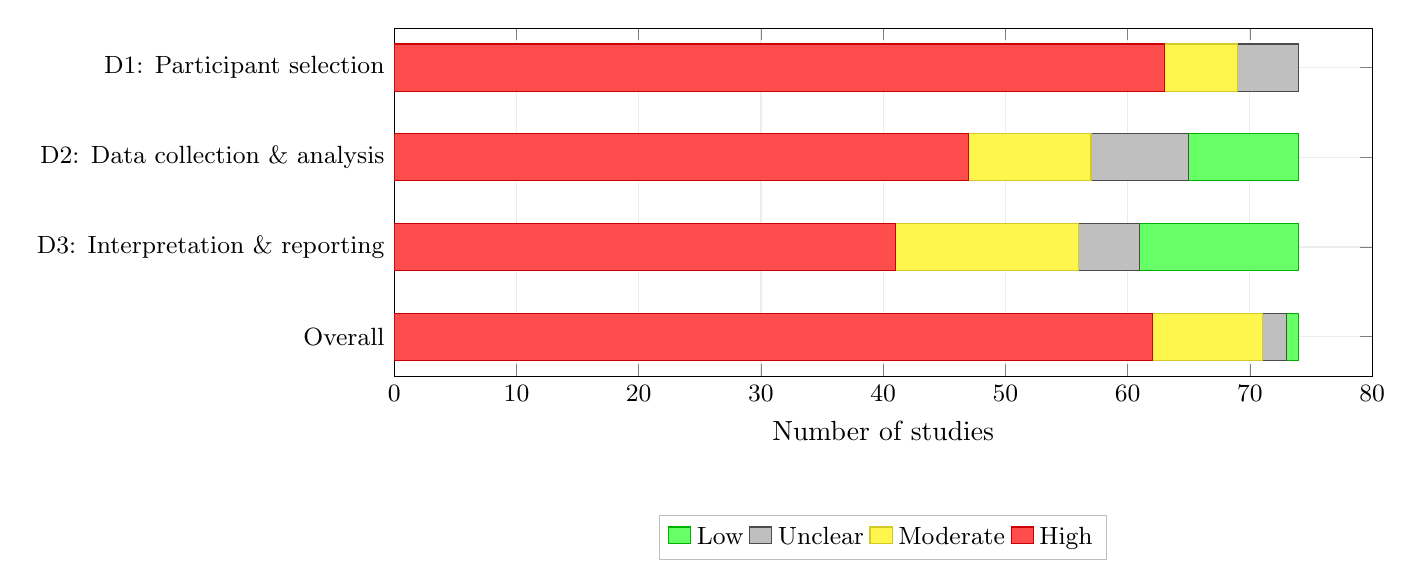
\begin{tikzpicture}
\begin{axis}[
    xbar stacked,
    width=14cm,
    height=6cm,
    xlabel={Number of studies},
    xmin=0, xmax=80,
    ytick=data,
    yticklabels={
        {Overall},
        {D3: Interpretation \& reporting},
        {D2: Data collection \& analysis},
        {D1: Participant selection}
    },
    yticklabel style={font=\small},
    xticklabel style={font=\small},
    legend style={at={(0.5,-0.40)}, anchor=north, legend columns=4,
        font=\small, draw=gray!50},
    bar width=0.6cm,
    enlarge y limits={abs=0.5cm},
    grid=major,
    grid style={gray!15, thin},
    xtick={0,10,20,30,40,50,60,70,80},
    reverse legend,
]
\addplot[fill=red!70, draw=red!80!black] coordinates {
    (62, 0) (41, 1) (47, 2) (63, 3)
};
\addplot[fill=yellow!70, draw=yellow!80!black] coordinates {
    (9, 0) (15, 1) (10, 2) (6, 3)
};
\addplot[fill=gray!50, draw=gray!60!black] coordinates {
    (2, 0) (5, 1) (8, 2) (5, 3)
};
\addplot[fill=green!60, draw=green!70!black] coordinates {
    (1, 0) (13, 1) (9, 2) (0, 3)
};
\legend{High, Moderate, Unclear, Low}
% Percentage labels on high-risk bars
\node[font=\scriptsize, text=white, anchor=east] at (axis cs:60, 0) {83.8\%};
\node[font=\scriptsize, text=white, anchor=east] at (axis cs:39, 1) {55.4\%};
\node[font=\scriptsize, text=white, anchor=east] at (axis cs:45, 2) {63.5\%};
\node[font=\scriptsize, text=white, anchor=east] at (axis cs:61, 3) {85.1\%};
\end{axis}
\end{tikzpicture}
\caption{Risk-of-bias ratings by domain and overall ($n = 74$). The gradient from Domain~1 (85.1\% high) to Domain~3 (55.4\% high) indicates that participant selection is the most persistent source of weakness, while interpretive practices are relatively stronger.}
\label{fig:rob-domains}
\end{figure}


\begin{figure}[!h]
\centering
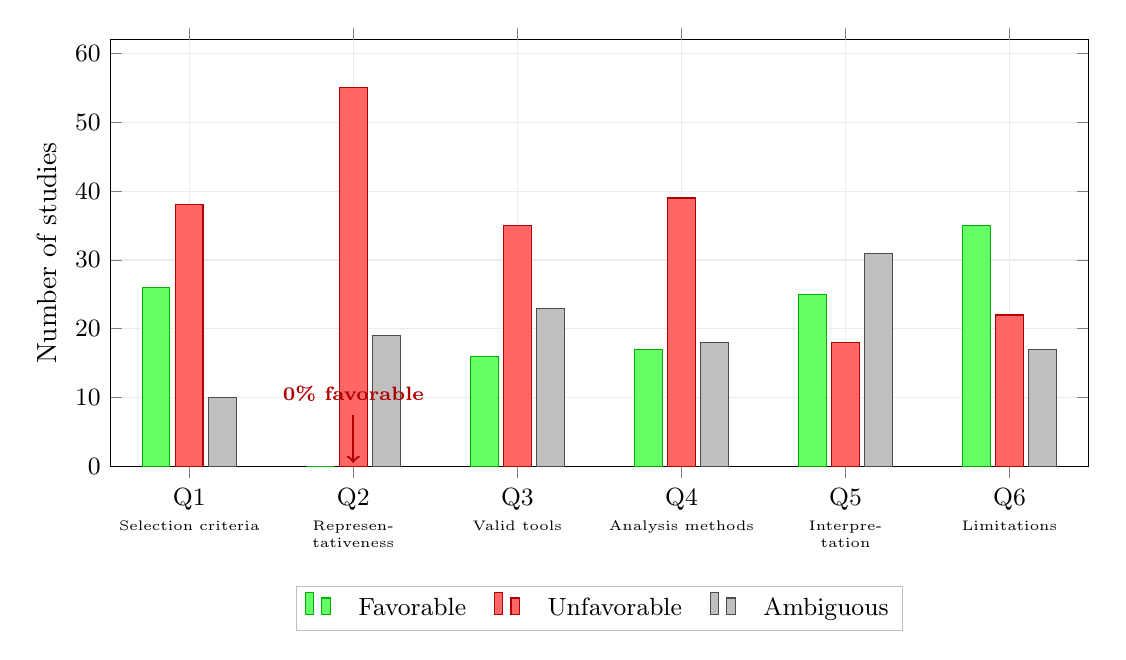
\begin{tikzpicture}
\begin{axis}[
    ybar,
    width=14cm,
    height=7cm,
    ylabel={Number of studies},
    ymin=0, ymax=62,
    symbolic x coords={Q1,Q2,Q3,Q4,Q5,Q6},
    xtick=data,
    xticklabel style={font=\small},
    yticklabel style={font=\small},
    bar width=0.35cm,
    enlarge x limits={abs=1cm},
    legend style={at={(0.5,-0.28)}, anchor=north, legend columns=3,
        font=\small, draw=gray!50, column sep=8pt, /tikz/every even column/.append style={column sep=8pt}},
    grid=major,
    grid style={gray!15, thin},
    ytick={0,10,20,30,40,50,60},
    % Extra x-axis labels below the Q codes
    extra x ticks={Q1,Q2,Q3,Q4,Q5,Q6},
    extra x tick style={
        xticklabel style={font=\tiny, anchor=north, yshift=-12pt, text width=2cm, align=center},
    },
    extra x tick labels={
        {Selection criteria},
        {Represen-\\tativeness},
        {Valid tools},
        {Analysis methods},
        {Interpre-\\tation},
        {Limitations}
    },
]
% Favorable (green)
\addplot[fill=green!60, draw=green!70!black] coordinates {
    (Q1, 26) (Q2, 0) (Q3, 16) (Q4, 17) (Q5, 25) (Q6, 35)
};
% Unfavorable (red)
\addplot[fill=red!60, draw=red!70!black] coordinates {
    (Q1, 38) (Q2, 55) (Q3, 35) (Q4, 39) (Q5, 18) (Q6, 22)
};
% Ambiguous (gray)
\addplot[fill=gray!50, draw=gray!60!black] coordinates {
    (Q1, 10) (Q2, 19) (Q3, 23) (Q4, 18) (Q5, 31) (Q6, 17)
};
\legend{Favorable, Unfavorable, Ambiguous}
% Callout annotation for Q2
\node[font=\scriptsize\bfseries, text=red!70!black, anchor=south] at (axis cs:Q2, 8) {0\% favorable};
\draw[->, thick, red!70!black] (axis cs:Q2, 7.5) -- (axis cs:Q2, 0.5);
\end{axis}
\end{tikzpicture}
\caption{Signalling question-level analysis of risk-of-bias assessments across 74 studies. Q2 (sample representativeness) received no favourable ratings --- the single most striking methodological finding in the corpus. Q6 (limitations discussed) achieved the highest favourable rate (47.3\%) (see Section~\ref{sec:rob-results}).}
\label{fig:signalling-questions}
\end{figure}


\begin{figure}[!h]
\centering
\resizebox{\textwidth}{!}{%
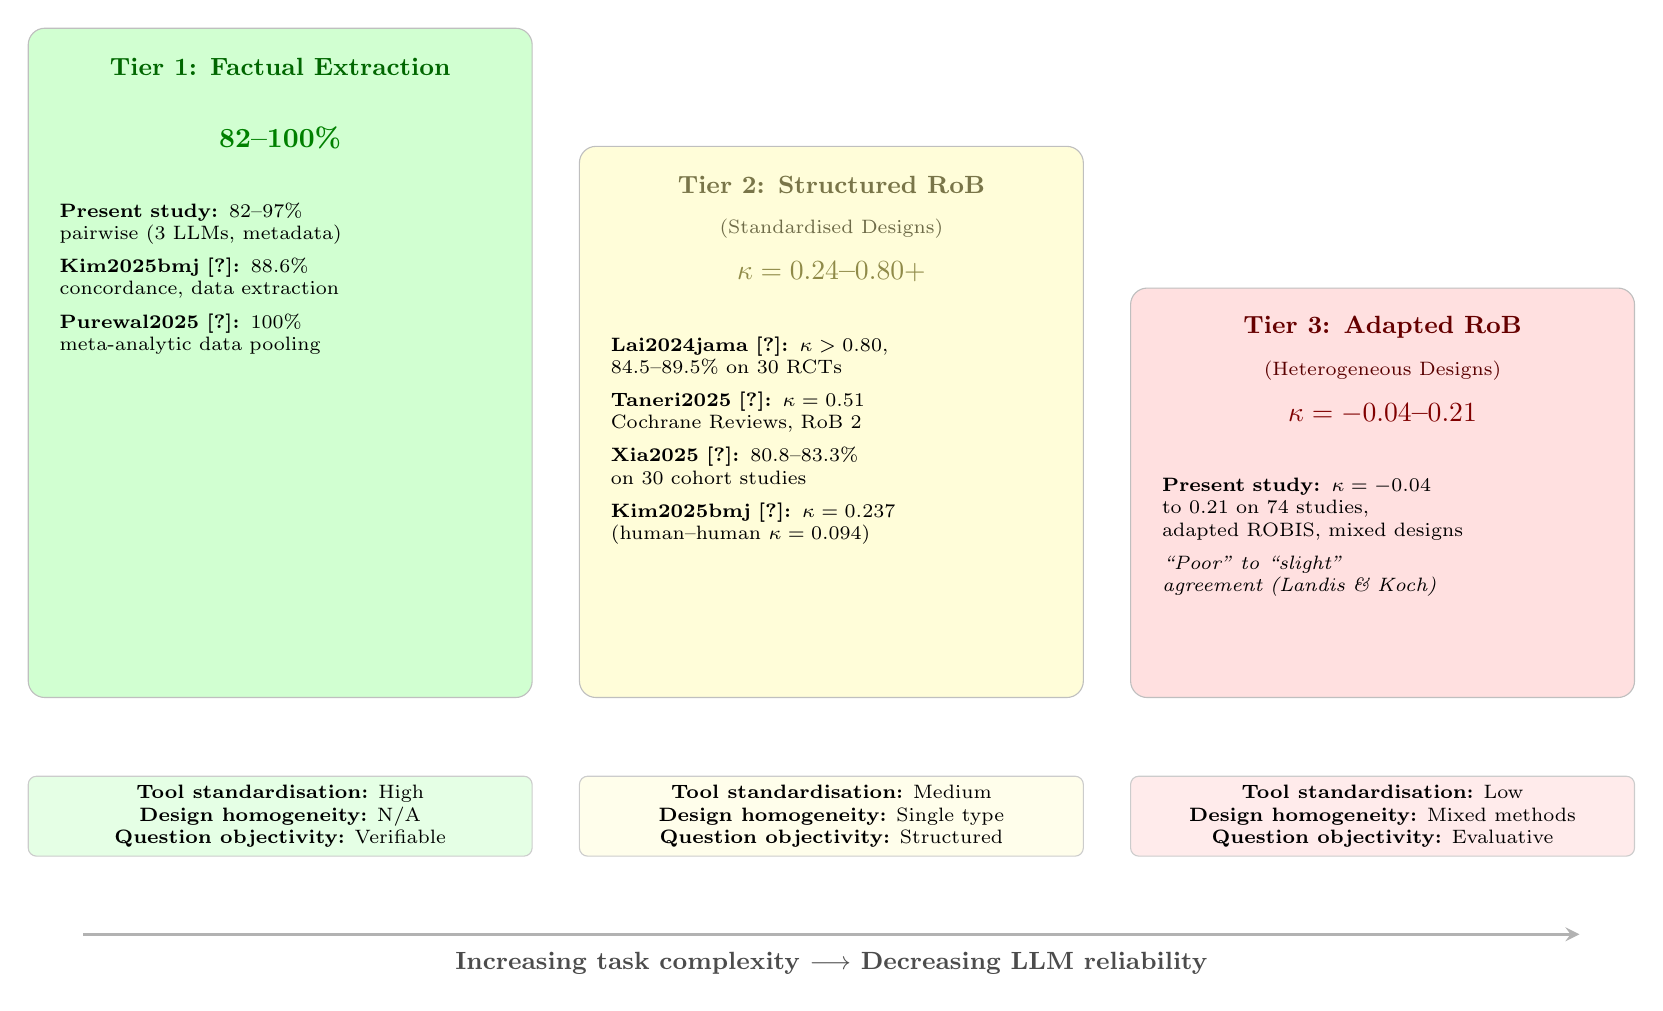
\begin{tikzpicture}[
  tierbox/.style={rectangle, draw=gray!50, rounded corners=6pt,
    minimum width=6.4cm, align=center, font=\small, inner sep=8pt},
  datapt/.style={font=\scriptsize, align=left, text width=5.6cm, anchor=north},
  factbox/.style={rectangle, draw=gray!40, rounded corners=3pt,
    fill=gray!8, minimum width=6.4cm, minimum height=0.8cm,
    align=center, font=\scriptsize},
  arrlabel/.style={font=\small\bfseries, text=black!70},
]

% Horizontal positions
\def\colA{0}
\def\colB{7.0}
\def\colC{14.0}

% Common bottom edge for all tier boxes
\def\ybottom{-3.0}

% ============================================================
% TIER 1 — green, tallest (7.0cm)
% ============================================================
\node[tierbox, fill=green!18, minimum height=8.5cm, anchor=south]
  (t1) at (\colA, \ybottom) {};
\node[font=\small\bfseries, text=green!40!black]
  at ([yshift=-0.5cm]t1.north) {Tier~1: Factual Extraction};
\node[font=\normalsize\bfseries, text=green!50!black]
  at ([yshift=-1.4cm]t1.north) {82--100\%};
\node[datapt] at ([yshift=-2.1cm]t1.north) {%
  \textbf{Present study:} 82--97\%\\pairwise (3~LLMs, metadata)\\[4pt]
  \textbf{\citeauthor{Kim2025bmj}~\cite{Kim2025bmj}:} 88.6\%\\concordance, data extraction\\[4pt]
  \textbf{\citeauthor{Purewal2025}~\cite{Purewal2025}:} 100\%\\meta-analytic data pooling};

% ============================================================
% TIER 2 — yellow, medium height (5.5cm)
% ============================================================
\node[tierbox, fill=yellow!15, minimum height=7.0cm, anchor=south]
  (t2) at (\colB, \ybottom) {};
\node[font=\small\bfseries, text=yellow!40!black]
  at ([yshift=-0.5cm]t2.north) {Tier~2: Structured RoB};
\node[font=\scriptsize, text=yellow!35!black]
  at ([yshift=-1.05cm]t2.north) {(Standardised Designs)};
\node[font=\normalsize\bfseries, text=yellow!50!black]
  at ([yshift=-1.6cm]t2.north) {$\kappa = 0.24$--$0.80+$};
\node[datapt] at ([yshift=-2.3cm]t2.north) {%
  \textbf{\citeauthor{Lai2024jama}~\cite{Lai2024jama}:} $\kappa > 0.80$,\\84.5--89.5\% on 30 RCTs\\[4pt]
  \textbf{\citeauthor{Taneri2025}~\cite{Taneri2025}:} $\kappa = 0.51$\\Cochrane Reviews, RoB~2\\[4pt]
  \textbf{\citeauthor{Xia2025}~\cite{Xia2025}:} 80.8--83.3\%\\on 30 cohort studies\\[4pt]
  \textbf{\citeauthor{Kim2025bmj}~\cite{Kim2025bmj}:} $\kappa = 0.237$\\(human--human $\kappa = 0.094$)};

% ============================================================
% TIER 3 — red, shortest (4.0cm)
% ============================================================
\node[tierbox, fill=red!12, minimum height=5.2cm, anchor=south]
  (t3) at (\colC, \ybottom) {};
\node[font=\small\bfseries, text=red!40!black]
  at ([yshift=-0.5cm]t3.north) {Tier~3: Adapted RoB};
\node[font=\scriptsize, text=red!35!black]
  at ([yshift=-1.05cm]t3.north) {(Heterogeneous Designs)};
\node[font=\normalsize\bfseries, text=red!50!black]
  at ([yshift=-1.6cm]t3.north) {$\kappa = -0.04$--$0.21$};
\node[datapt] at ([yshift=-2.3cm]t3.north) {%
  \textbf{Present study:} $\kappa = -0.04$\\to $0.21$ on 74 studies,\\adapted ROBIS, mixed designs\\[4pt]
  {\itshape``Poor'' to ``slight''\\agreement (Landis \& Koch)}};

% ============================================================
% THREE-FACTOR MODEL (below tiers)
% ============================================================
\def\yfact{-4.5}

\node[factbox, fill=green!10] at (\colA, \yfact) {%
  \textbf{Tool standardisation:} High\\
  \textbf{Design homogeneity:} N/A\\
  \textbf{Question objectivity:} Verifiable};

\node[factbox, fill=yellow!8] at (\colB, \yfact) {%
  \textbf{Tool standardisation:} Medium\\
  \textbf{Design homogeneity:} Single type\\
  \textbf{Question objectivity:} Structured};

\node[factbox, fill=red!8] at (\colC, \yfact) {%
  \textbf{Tool standardisation:} Low\\
  \textbf{Design homogeneity:} Mixed methods\\
  \textbf{Question objectivity:} Evaluative};

% ============================================================
% BOTTOM ARROW
% ============================================================
\draw[->, >=stealth, very thick, draw=gray!60]
  (\colA - 2.5, -6.0) -- (\colC + 2.5, -6.0);
\node[arrlabel, below] at ({\colB}, -6.1)
  {Increasing task complexity $\longrightarrow$ Decreasing LLM reliability};

\end{tikzpicture}%
}% end resizebox
\caption{The task complexity gradient in LLM-assisted systematic review. LLM reliability decreases predictably from factual extraction (Tier~1) through structured risk-of-bias assessment on standardised designs (Tier~2) to adapted risk-of-bias assessment on heterogeneous educational studies (Tier~3). Data points from the present study (bold) are contextualised against published benchmarks. The gradient is driven by three interacting factors: tool standardisation, study design homogeneity, and question objectivity (see Section~\ref{sec:llm-validation}).}
\label{fig:llm-reliability-gradient}
\end{figure}


\begin{figure}[htbp]
\centering
\resizebox{\textwidth}{!}{%
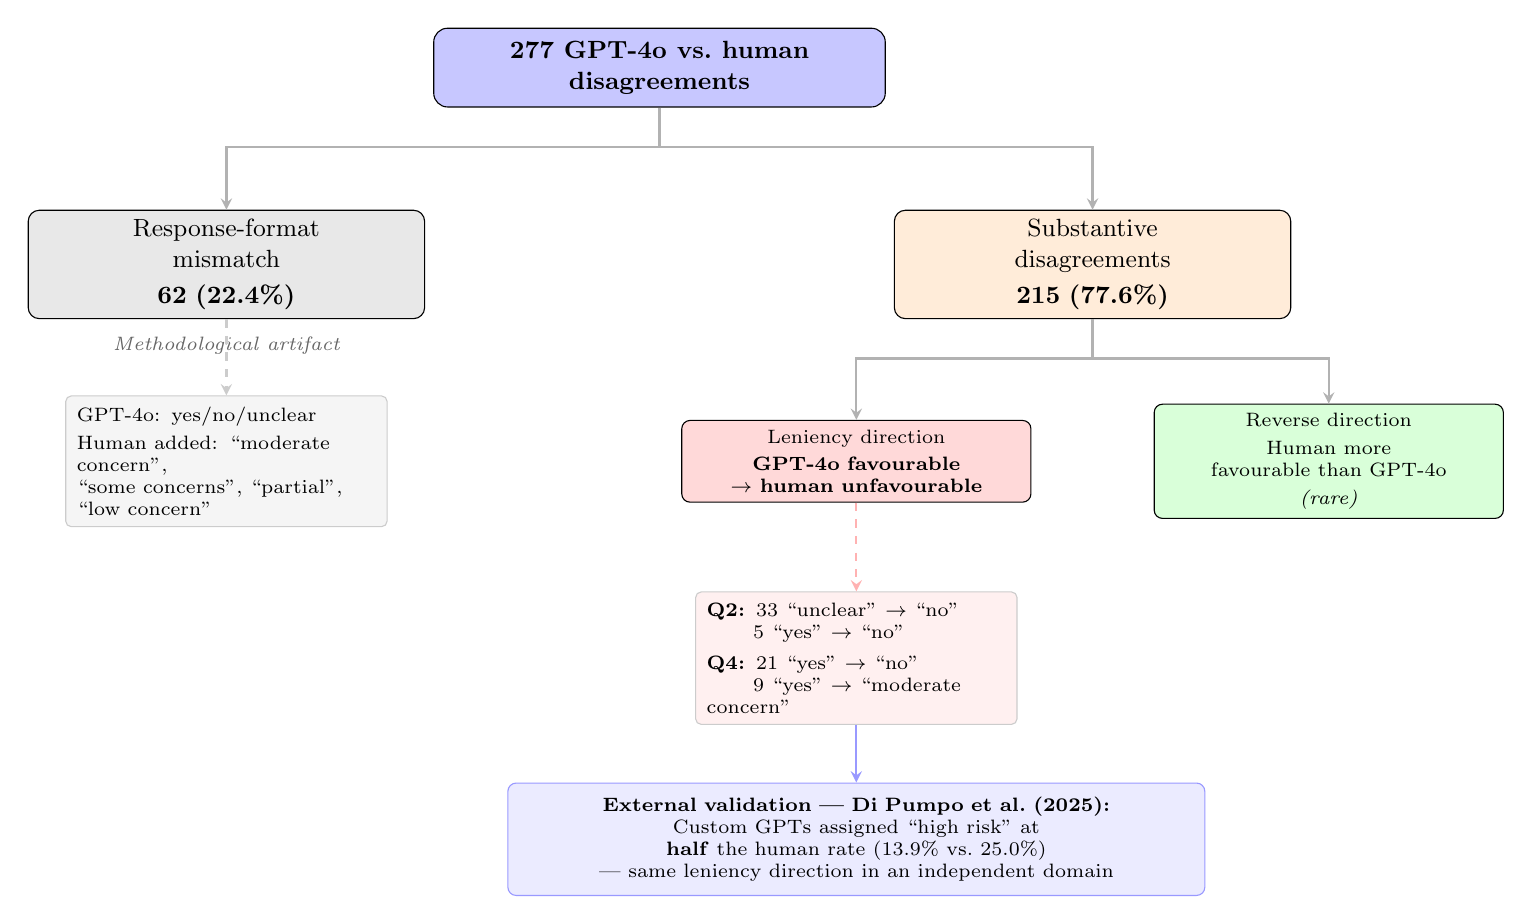
\begin{tikzpicture}[
  rootbox/.style={rectangle, draw, rounded corners=5pt, fill=blue!22,
    text width=5.5cm, minimum height=1.0cm, align=center, font=\small\bfseries},
  catbox/.style={rectangle, draw, rounded corners=4pt,
    text width=4.8cm, minimum height=0.9cm, align=center, font=\small},
  subbox/.style={rectangle, draw, rounded corners=3pt,
    text width=4.2cm, minimum height=0.8cm, align=center, font=\scriptsize},
  exbox/.style={rectangle, draw=gray!40, rounded corners=2pt, fill=white,
    text width=3.8cm, align=left, font=\scriptsize, inner sep=4pt},
  valbox/.style={rectangle, draw=blue!40, rounded corners=3pt, fill=blue!8,
    text width=8.5cm, align=center, font=\scriptsize, inner sep=5pt},
  ann/.style={font=\scriptsize\itshape, text=black!60},
  arr/.style={->, >=stealth, thick, draw=gray!60},
]

% ============================================================
% ROOT NODE
% ============================================================
\node[rootbox] (root) at (0, 0) {277 GPT-4o vs.\ human\\disagreements};

% ============================================================
% BRANCH A: Response-format mismatch
% ============================================================
\node[catbox, fill=gray!18] (fmatch) at (-5.5, -2.5) {Response-format\\mismatch\\[2pt]\textbf{62 (22.4\%)}};
\node[ann, anchor=north] at (-5.5, -3.3) {Methodological artifact};

% ============================================================
% BRANCH B: Substantive disagreements
% ============================================================
\node[catbox, fill=orange!15] (subst) at (5.5, -2.5) {Substantive\\disagreements\\[2pt]\textbf{215 (77.6\%)}};

% Arrows from root
\draw[arr] (root.south) -- ++(0, -0.5) -| (fmatch.north);
\draw[arr] (root.south) -- ++(0, -0.5) -| (subst.north);

% ============================================================
% Format mismatch detail
% ============================================================
\node[exbox, fill=gray!8] (fmdet) at (-5.5, -5.0) {%
  GPT-4o: yes/no/unclear\\[2pt]
  Human added: ``moderate concern'',\\
  ``some concerns'', ``partial'',\\
  ``low concern''};
\draw[arr, dashed, draw=gray!40] (fmatch.south) -- (fmdet.north);

% ============================================================
% BRANCH B1: Leniency direction (dominant)
% ============================================================
\node[subbox, fill=red!15] (leniency) at (2.5, -5.0) {Leniency direction\\[2pt]\textbf{GPT-4o favourable}\\$\rightarrow$ \textbf{human unfavourable}};

% ============================================================
% BRANCH B2: Reverse direction (minor)
% ============================================================
\node[subbox, fill=green!15] (reverse) at (8.5, -5.0) {Reverse direction\\[2pt]Human more\\favourable than GPT-4o\\[2pt]{\itshape(rare)}};

% Arrows from substantive
\draw[arr] (subst.south) -- ++(0, -0.5) -| (leniency.north);
\draw[arr] (subst.south) -- ++(0, -0.5) -| (reverse.north);

% ============================================================
% Leniency examples
% ============================================================
\node[exbox, fill=red!6] (lex) at (2.5, -7.5) {%
  \textbf{Q2:} 33 ``unclear'' $\rightarrow$ ``no''\\
  \hspace{2.1em}5 ``yes'' $\rightarrow$ ``no''\\[3pt]
  \textbf{Q4:} 21 ``yes'' $\rightarrow$ ``no''\\
  \hspace{2.1em}9 ``yes'' $\rightarrow$ ``moderate concern''};
\draw[arr, dashed, draw=red!30] (leniency.south) -- (lex.north);

% ============================================================
% EXTERNAL VALIDATION
% ============================================================
\node[valbox] (extval) at (2.5, -9.8) {%
  \textbf{External validation --- Di~Pumpo et al.\ (2025):}\\
  Custom GPTs assigned ``high risk'' at \textbf{half} the human rate (13.9\% vs.\ 25.0\%)\\
  --- same leniency direction in an independent domain};
\draw[arr, draw=blue!40] (lex.south) -- (extval.north);

\end{tikzpicture}%
}% end resizebox
\caption{Taxonomy of the 277 disagreements between GPT-4o and human-verified risk-of-bias assessments. Response-format mismatches (22.4\%) inflate measured disagreement without reflecting substantive differences. Among substantive disagreements, the dominant pattern is leniency bias: GPT-4o systematically applied less stringent criteria than human reviewers, consistent with independent findings by Di~Pumpo et~al.~(2025).}
\label{fig:disagreement-taxonomy}
\end{figure}


\begin{figure}[!h]
\centering
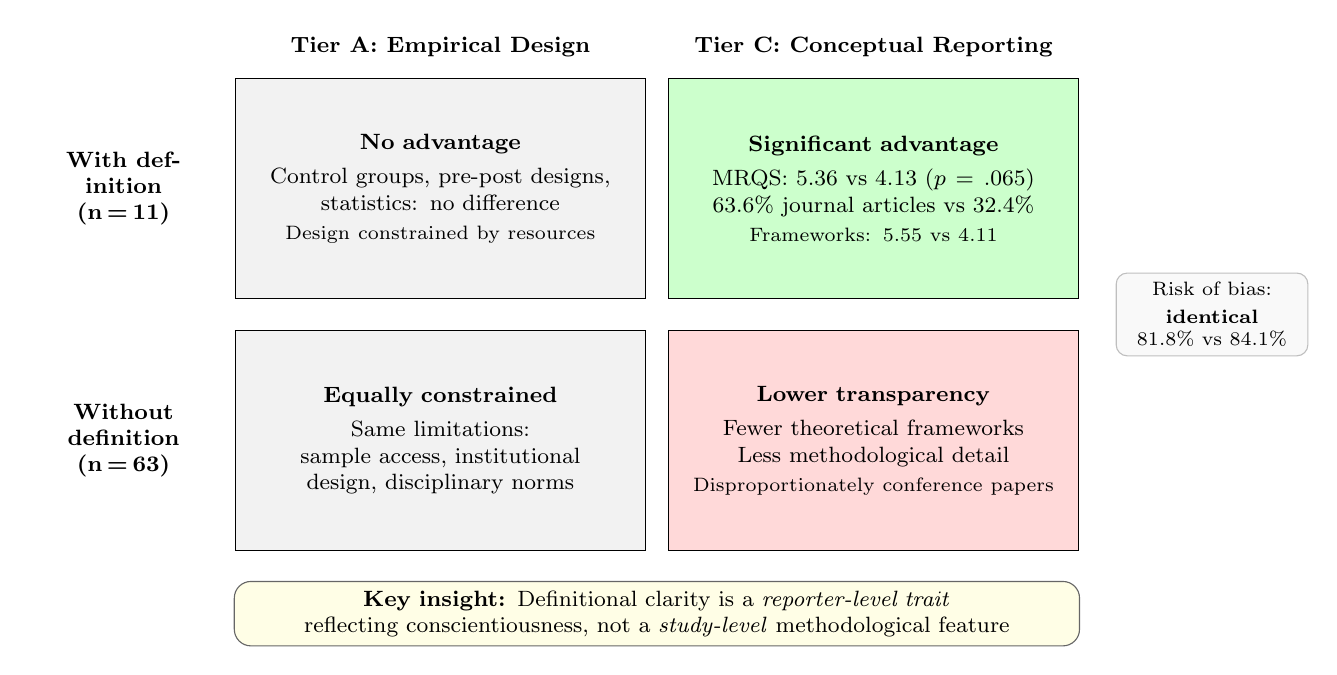
\begin{tikzpicture}[
  cell/.style={
    draw, minimum width=5.2cm, minimum height=2.8cm,
    text width=4.7cm, align=center, font=\footnotesize
  },
  header/.style={
    font=\footnotesize\bfseries, align=center
  },
]

% Column headers
\node[header] at (2.6, 1.8) {Tier~A: Empirical Design};
\node[header] at (8.1, 1.8) {Tier~C: Conceptual Reporting};

% Row headers — anchored east, clear of cells
\node[header, text width=2.2cm, anchor=east] at (-0.2, 0) {With definition\\(n\,=\,11)};
\node[header, text width=2.2cm, anchor=east] at (-0.2, -3.2) {Without definition\\(n\,=\,63)};

% Top-left: With definition × Tier A
\node[cell, fill=gray!10] (tl) at (2.6, 0) {%
  \textbf{No advantage}\\[3pt]
  Control groups, pre-post designs,\\
  statistics: no difference\\[1pt]
  {\scriptsize Design constrained by resources}%
};

% Top-right: With definition × Tier C
\node[cell, fill=green!20] (tr) at (8.1, 0) {%
  \textbf{Significant advantage}\\[3pt]
  MRQS: 5.36 vs 4.13 ($p = .065$)\\
  63.6\% journal articles vs 32.4\%\\[1pt]
  {\scriptsize Frameworks: 5.55 vs 4.11}%
};

% Bottom-left: Without definition × Tier A
\node[cell, fill=gray!10] (bl) at (2.6, -3.2) {%
  \textbf{Equally constrained}\\[3pt]
  Same limitations:\\
  sample access, institutional\\
  design, disciplinary norms%
};

% Bottom-right: Without definition × Tier C
\node[cell, fill=red!15] (br) at (8.1, -3.2) {%
  \textbf{Lower transparency}\\[3pt]
  Fewer theoretical frameworks\\
  Less methodological detail\\[1pt]
  {\scriptsize Disproportionately conference papers}%
};

% Right annotation: RoB
\node[
  draw=gray!50, rounded corners=4pt, fill=gray!5,
  text width=2.2cm, align=center, font=\scriptsize
] at (12.4, -1.6) {%
  Risk of bias:\\[2pt]
  \textbf{identical}\\
  81.8\% vs 84.1\%%
};

% Bottom insight box
\node[
  draw=black!60, rounded corners=6pt, fill=yellow!10,
  text width=10.5cm, align=center, font=\footnotesize
] at (5.35, -5.4) {%
  \textbf{Key insight:} Definitional clarity is a \emph{reporter-level trait}\\
  reflecting conscientiousness, not a \emph{study-level} methodological feature%
};

\end{tikzpicture}
\caption{Interaction between definitional practices and quality dimensions. Studies with explicit definitions score higher on conceptual reporting items (Tier~C, right column) but show no advantage on empirical design items (Tier~A, left column). Risk of bias is effectively identical regardless of definitional practices. This pattern reveals that definitional clarity operates as a reporter-level trait reflecting conscientiousness, not as a driver of stronger study design (see Section~\ref{sec:def-quality}).}
\label{fig:definitional-quality-interaction}
\end{figure}


\begin{figure}[htbp]
\centering
\resizebox{\textwidth}{!}{%
\begin{tikzpicture}[
  stage/.style={
    draw, rounded corners=6pt, minimum width=11cm, minimum height=1.6cm,
    text width=10.5cm, align=center, font=\small
  },
  annotation/.style={
    text width=5.5cm, align=left, font=\footnotesize\itshape
  },
  arrow/.style={-{Stealth[length=5pt]}, thick},
  breakline/.style={dashed, thick, red!60!black},
]

% Stage 1
\node[stage, fill=orange!20] (s1) at (0, 0) {%
  \textbf{Stage~1: Definitional Ambiguity}\\[2pt]
  85.1\% of studies provide no explicit definition%
};
\node[annotation, right] at (s1.east) {%
  \hspace{6pt}$\geq$4 distinct constructs\\
  \hspace{6pt}under one label%
};

% Stage 2
\node[stage, fill=orange!25] (s2) at (0, -2.6) {%
  \textbf{Stage~2: Construct Heterogeneity}\\[2pt]
  Different interventions share the same name%
};
\node[annotation, right] at (s2.east) {%
  \hspace{6pt}structural, content,\\
  \hspace{6pt}full, GBL%
};

% Stage 3
\node[stage, fill=red!15] (s3) at (0, -5.2) {%
  \textbf{Stage~3: Measurement Incommensurability}\\[2pt]
  21.6\% validated instruments; 9.5\% report effect sizes%
};
\node[annotation, right] at (s3.east) {%
  \hspace{6pt}ad hoc measures,\\
  \hspace{6pt}incomparable outcomes%
};

% Stage 4
\node[stage, fill=red!20] (s4) at (0, -7.8) {%
  \textbf{Stage~4: Synthesis Failure}\\[2pt]
  Meta-analysis structurally foreclosed%
};
\node[annotation, right] at (s4.east) {%
  \hspace{6pt}narrative synthesis only%
};

% Stage 5
\node[stage, fill=red!25] (s5) at (0, -10.4) {%
  \textbf{Stage~5: Knowledge Gap Persistence}\\[2pt]
  20 years, 74 studies, no converged answer%
};
\node[annotation, right] at (s5.east) {%
  \hspace{6pt}pre-paradigmatic\\
  \hspace{6pt}accumulation%
};

% Arrows between stages
\draw[arrow] (s1.south) -- (s2.north);
\draw[arrow] (s2.south) -- (s3.north);
\draw[arrow] (s3.south) -- (s4.north);
\draw[arrow] (s4.south) -- (s5.north);

% Intervention point — left side
\draw[breakline] (-7.2, 0.9) -- (-7.2, -1.0);
\node[
  draw=red!60!black, rounded corners=4pt, fill=yellow!15,
  text width=3.2cm, align=center, font=\footnotesize\bfseries,
  left
] at (-7.4, 0) {%
  INTERVENTION\\POINT:\\[2pt]
  Require explicit\\definitions%
};
\draw[breakline, -{Stealth[length=4pt]}] (-7.2, 0) -- (s1.west);

% Bottom note
\node[
  draw=gray!50, rounded corners=4pt, fill=gray!5,
  text width=13cm, align=center, font=\small
] at (0, -12.4) {%
  Breaking the cascade at Stage~1 would propagate improvements\\
  through all subsequent stages%
};

\end{tikzpicture}%
}
\caption{The construct validity cascade in gamification-in-history research. Definitional ambiguity (Stage~1) propagates through construct heterogeneity (Stage~2), measurement incommensurability (Stage~3), and synthesis failure (Stage~4) to perpetuate knowledge gaps (Stage~5). Each stage is quantitatively anchored to findings from the 74-study corpus. The cascade can be interrupted at Stage~1 through explicit definitional requirements.}
\label{fig:construct-validity-cascade}
\end{figure}


\begin{figure}[!h]
\centering
\resizebox{0.9\textwidth}{!}{%
\begin{tikzpicture}[
  statconc/.style={rectangle, rounded corners=6pt, draw=blue!50, fill=blue!22,
    text width=3.2cm, minimum height=1.4cm, align=center, font=\small\bfseries,
    line width=0.8pt},
  internal/.style={rectangle, rounded corners=6pt, draw=orange!60, fill=orange!15,
    text width=3.2cm, minimum height=1.4cm, align=center, font=\small\bfseries,
    line width=0.8pt},
  external/.style={rectangle, rounded corners=6pt, draw=red!60, fill=red!15,
    text width=3.2cm, minimum height=1.4cm, align=center, font=\small\bfseries,
    line width=0.8pt},
  construct/.style={rectangle, rounded corners=6pt, draw=purple!50, fill=purple!10,
    text width=3.2cm, minimum height=1.4cm, align=center, font=\small\bfseries,
    line width=0.8pt},
  arr/.style={->, >=stealth, thick, draw=gray!70},
  lbl/.style={font=\scriptsize, text=gray!50!black, fill=white, inner sep=2pt},
  annot/.style={font=\scriptsize\itshape, text=gray!60, text width=3.2cm, align=center},
]

% Diamond layout: top, right, bottom, left
\node[statconc] (sc) at (0, 4.2) {Statistical\\Conclusion\\Validity};
\node[annot, right=4pt of sc] (sc-a) {66.1\% underpowered\\90.5\% no effect sizes};

\node[internal] (iv) at (5.2, 0) {Internal\\Validity};
\node[annot, below=1pt of iv] (iv-a) {31\% no control\\confounding, novelty};

\node[external] (ev) at (0, -4.2) {External\\Validity};
\node[annot, below=1pt of ev] (ev-a) {Q2: 0\% favourable\\55.4\% in 4 countries};

\node[construct] (cv) at (-5.2, 0) {Construct\\Validity};
\node[annot, below=1pt of cv] (cv-a) {21.6\% validated\\85.1\% no definition};

% Directed arrows with interaction labels
\draw[arr] (sc) to[bend right=15]
  node[lbl, pos=0.45, anchor=south west] {inflated effects}
  (iv);
\draw[arr] (cv) to[bend right=15]
  node[lbl, pos=0.45, anchor=south east] {wrong construct measured}
  (sc);
\draw[arr] (cv) to[bend left=15]
  node[lbl, pos=0.5, anchor=south] {cannot distinguish treatment}
  (iv);
\draw[arr] (iv) to[bend right=15]
  node[lbl, pos=0.45, anchor=north west] {cannot generalise valid effects}
  (ev);
\draw[arr] (ev) to[bend right=15]
  node[lbl, pos=0.45, anchor=north east] {culturally-specific instruments}
  (cv);

% Central annotation
\node[draw=red!60!black, fill=yellow!12, rounded corners=5pt,
  font=\small\bfseries, text=red!70!black, inner sep=8pt,
  line width=0.8pt, text width=3.8cm, align=center]
  at (0, 0)
  {Evidence certainty:\\Very Low};

\end{tikzpicture}%
}% end resizebox
\caption{Bias interaction network: directed pathways between validity threats in the 74-study corpus. Each arrow represents a mechanism by which weakness in one validity type amplifies weakness in another. The co-occurrence of all four threats (43.2\% of studies rated high risk across all three ROBIS domains vs.\ 29.9\% expected under independence) produces cumulative evidence certainty of Very Low (see Section~\ref{sec:detailed-bias}).}
\label{fig:bias-interaction-network}
\end{figure}


\begin{figure}[htbp]
\centering
\resizebox{\textwidth}{!}{%
\begin{tikzpicture}[
  startbox/.style={
    draw=green!60!black, rounded corners=6pt, fill=green!12,
    minimum width=2.4cm, minimum height=1.6cm, align=center,
    font=\small\bfseries, line width=0.8pt
  },
  downgrade/.style={
    draw, rounded corners=6pt, minimum width=2.2cm, minimum height=2.0cm,
    align=center, font=\small, line width=0.8pt
  },
  finalbox/.style={
    draw=red!70!black, rounded corners=6pt, fill=red!25,
    minimum width=2.4cm, minimum height=1.6cm, align=center,
    font=\small\bfseries, line width=0.8pt
  },
  arrow/.style={-{Stealth[length=5pt]}, thick, draw=gray!70},
  domainrow/.style={
    draw=gray!40, rounded corners=4pt, fill=gray!5,
    minimum width=2.0cm, minimum height=0.7cm, align=center,
    font=\scriptsize, line width=0.5pt
  },
  domainlabel/.style={
    text width=3.0cm, align=right, font=\scriptsize\itshape
  },
  domainfinal/.style={
    draw=red!50, rounded corners=3pt, fill=red!12,
    minimum width=1.8cm, minimum height=0.7cm, align=center,
    font=\scriptsize\bfseries, line width=0.5pt
  },
]

% Starting point
\node[startbox] (start) at (0, 0) {Low\\{\footnotesize(observational)}};

% Five downgrading boxes
\node[downgrade, fill=red!15] (d1) at (3.4, 0) {%
  \textbf{Risk of bias}\\[2pt]
  {\footnotesize 83.8\% high}\\[1pt]
  {\scriptsize$\downarrow$ Serious}%
};
\node[downgrade, fill=red!15] (d2) at (6.4, 0) {%
  \textbf{Inconsistency}\\[2pt]
  {\footnotesize Heterogeneous}\\{\footnotesize outcomes}\\[1pt]
  {\scriptsize$\downarrow$ Serious}%
};
\node[downgrade, fill=red!15] (d3) at (9.4, 0) {%
  \textbf{Indirectness}\\[2pt]
  {\footnotesize Construct}\\{\footnotesize ambiguity}\\[1pt]
  {\scriptsize$\downarrow$ Serious}%
};
\node[downgrade, fill=red!20] (d4) at (12.4, 0) {%
  \textbf{Imprecision}\\[2pt]
  {\footnotesize Median $n=34$}\\[1pt]
  {\scriptsize$\downarrow$ Very serious}%
};
\node[downgrade, fill=orange!15] (d5) at (15.4, 0) {%
  \textbf{Publication}\\{\textbf{bias}}\\[2pt]
  {\footnotesize Suspected}\\[1pt]
  {\scriptsize$\downarrow$}%
};

% Final box
\node[finalbox] (final) at (18.4, 0) {Very Low};

% Arrows in cascade
\draw[arrow] (start) -- (d1);
\draw[arrow] (d1) -- (d2);
\draw[arrow] (d2) -- (d3);
\draw[arrow] (d3) -- (d4);
\draw[arrow] (d4) -- (d5);
\draw[arrow] (d5) -- (final);

% Outcome domain rows below
\node[font=\small\bfseries, anchor=east] at (-0.8, -2.5) {Outcome domains:};

% Row labels
\node[domainlabel] at (-0.3, -3.5) {Engagement /\\Motivation};
\node[domainlabel] at (-0.3, -4.5) {Knowledge\\acquisition};
\node[domainlabel] at (-0.3, -5.5) {Historical\\thinking};
\node[domainlabel] at (-0.3, -6.5) {Long-term\\retention};

% Domain assessment cells — all arrive at Very Low
\foreach \y/\rob/\inc/\ind/\imp/\pub in {
  -3.5/Serious/No downgrade/Serious/Very serious/Suspected,
  -4.5/Serious/Serious/Serious/Very serious/Suspected,
  -5.5/Serious/N{/}A/Serious/Very serious/N{/}A,
  -6.5/Serious/N{/}A/Serious/Very serious/N{/}A%
}{
  \node[domainrow] at (3.4, \y) {\rob};
  \node[domainrow] at (6.4, \y) {\inc};
  \node[domainrow] at (9.4, \y) {\ind};
  \node[domainrow] at (12.4, \y) {\imp};
  \node[domainrow] at (15.4, \y) {\pub};
  \node[domainfinal] at (18.4, \y) {Very Low};
}

% Connecting dashed lines from cascade to domain rows
\foreach \x in {3.4, 6.4, 9.4, 12.4, 15.4, 18.4}{
  \draw[dashed, gray!40] (\x, -1.2) -- (\x, -2.2);
}

\end{tikzpicture}%
}% end resizebox
\caption{Evidence certainty assessment for gamification-in-history-education outcomes using a modified GRADE approach adapted for narrative synthesis (per SWiM Item~9, Campbell et~al.~2020). Starting from the baseline of Low for observational studies, systematic downgrading for risk of bias, inconsistency, indirectness, imprecision, and suspected publication bias produces Very Low certainty across all outcome domains.}
\label{fig:evidence-certainty-grade}
\end{figure}


\begin{figure}[htbp]
\centering
\resizebox{\textwidth}{!}{%
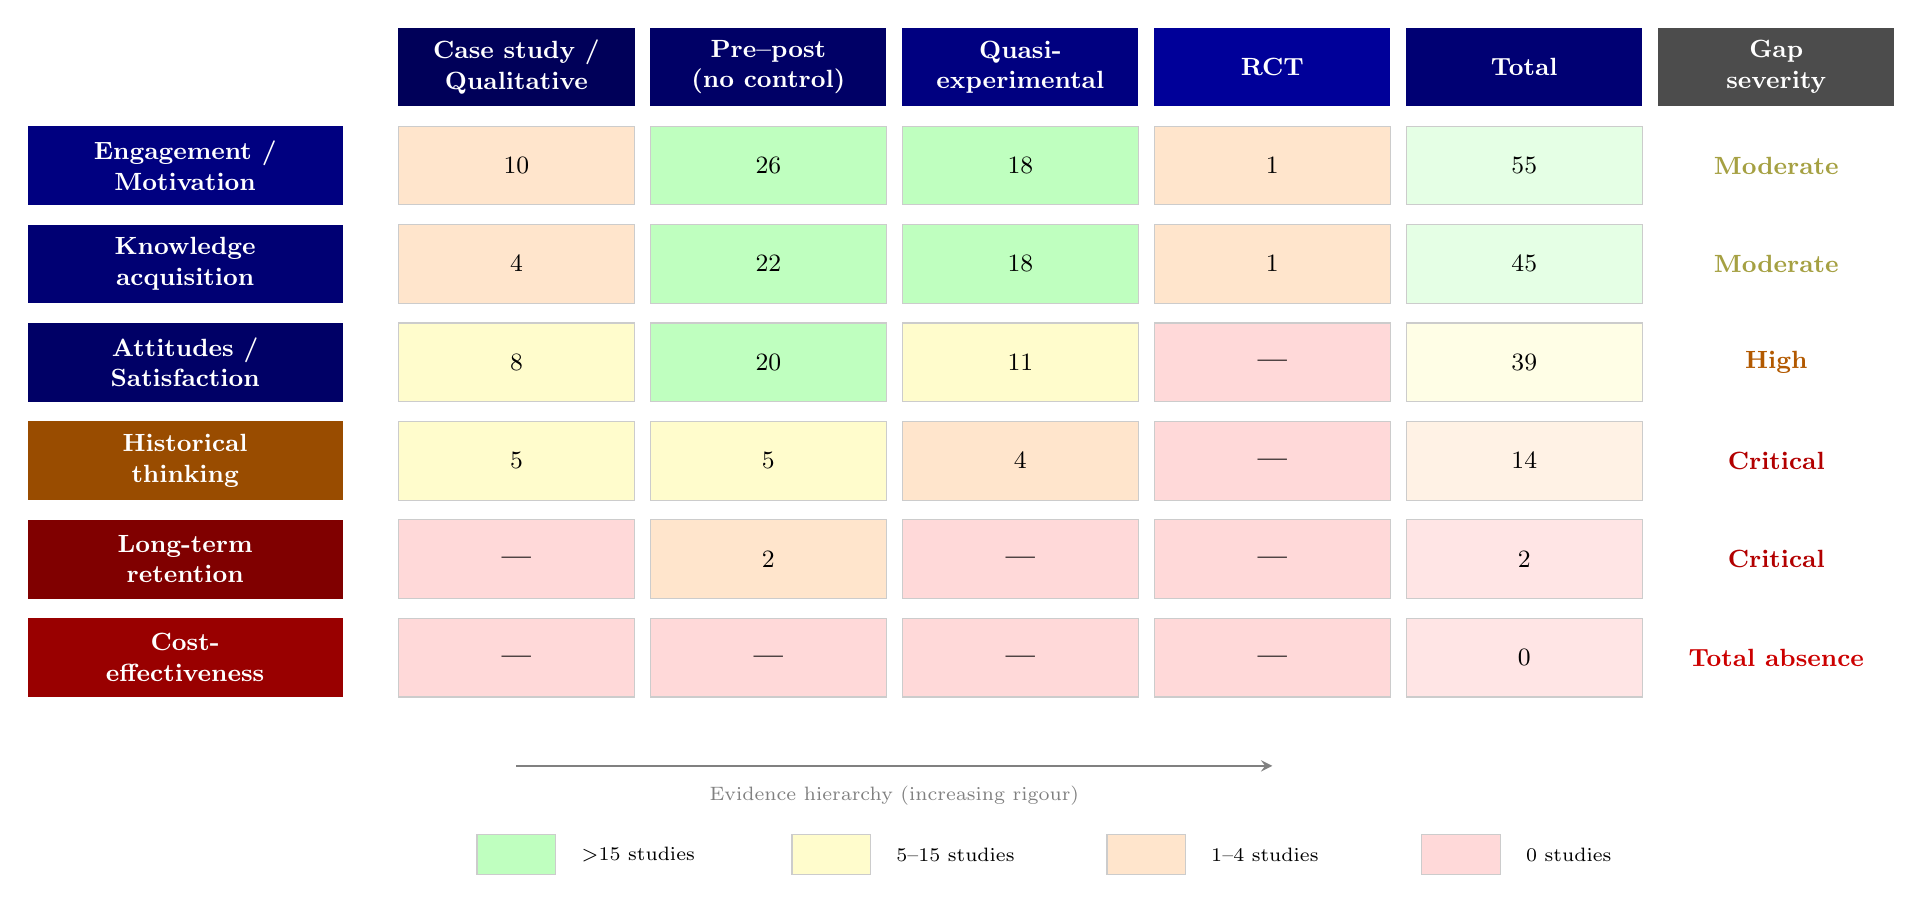
\begin{tikzpicture}[
  hdr/.style={font=\small\bfseries, text=white, minimum height=1.0cm,
    minimum width=3.0cm, align=center},
  rhdr/.style={font=\small\bfseries, text=white, minimum height=1.0cm,
    minimum width=4.0cm, align=center, anchor=east},
  cell/.style={rectangle, draw=gray!40, minimum height=1.0cm,
    minimum width=3.0cm, align=center, font=\small},
  dense/.style={cell, fill=green!25},
  moderate/.style={cell, fill=yellow!20},
  sparse/.style={cell, fill=orange!20},
  empty/.style={cell, fill=red!15, font=\small\bfseries},
  gap/.style={font=\small\bfseries, minimum height=1.0cm,
    minimum width=3.2cm, align=center},
]

% Column spacing
\def\colw{3.2}

% Column headers
\node[hdr, fill=blue!35!black] at (0, 0) {Case study /\\Qualitative};
\node[hdr, fill=blue!40!black] at (\colw, 0) {Pre--post\\(no control)};
\node[hdr, fill=blue!50!black] at (2*\colw, 0) {Quasi-\\experimental};
\node[hdr, fill=blue!60!black] at (3*\colw, 0) {RCT};
\node[hdr, fill=blue!45!black] at (4*\colw, 0) {Total};
\node[hdr, fill=gray!60!black] at (5*\colw, 0) {Gap\\severity};

% Row spacing
\def\rowh{1.25}

% Row 1: Engagement / Motivation
\node[rhdr, fill=blue!50!black] at (-2.2, -\rowh) {Engagement /\\Motivation};
\node[sparse] at (0, -\rowh) {10};
\node[dense] at (\colw, -\rowh) {26};
\node[dense] at (2*\colw, -\rowh) {18};
\node[sparse] at (3*\colw, -\rowh) {1};
\node[cell, fill=green!10] at (4*\colw, -\rowh) {55};
\node[gap, text=yellow!60!black] at (5*\colw, -\rowh) {Moderate};

% Row 2: Knowledge acquisition
\node[rhdr, fill=blue!45!black] at (-2.2, -2*\rowh) {Knowledge\\acquisition};
\node[sparse] at (0, -2*\rowh) {4};
\node[dense] at (\colw, -2*\rowh) {22};
\node[dense] at (2*\colw, -2*\rowh) {18};
\node[sparse] at (3*\colw, -2*\rowh) {1};
\node[cell, fill=green!10] at (4*\colw, -2*\rowh) {45};
\node[gap, text=yellow!60!black] at (5*\colw, -2*\rowh) {Moderate};

% Row 3: Attitudes / Satisfaction
\node[rhdr, fill=blue!40!black] at (-2.2, -3*\rowh) {Attitudes /\\Satisfaction};
\node[moderate] at (0, -3*\rowh) {8};
\node[dense] at (\colw, -3*\rowh) {20};
\node[moderate] at (2*\colw, -3*\rowh) {11};
\node[empty] at (3*\colw, -3*\rowh) {---};
\node[cell, fill=yellow!10] at (4*\colw, -3*\rowh) {39};
\node[gap, text=orange!70!black] at (5*\colw, -3*\rowh) {High};

% Row 4: Historical thinking
\node[rhdr, fill=orange!60!black] at (-2.2, -4*\rowh) {Historical\\thinking};
\node[moderate] at (0, -4*\rowh) {5};
\node[moderate] at (\colw, -4*\rowh) {5};
\node[sparse] at (2*\colw, -4*\rowh) {4};
\node[empty] at (3*\colw, -4*\rowh) {---};
\node[cell, fill=orange!10] at (4*\colw, -4*\rowh) {14};
\node[gap, text=red!70!black] at (5*\colw, -4*\rowh) {Critical};

% Row 5: Long-term retention
\node[rhdr, fill=red!50!black] at (-2.2, -5*\rowh) {Long-term\\retention};
\node[empty] at (0, -5*\rowh) {---};
\node[sparse] at (\colw, -5*\rowh) {2};
\node[empty] at (2*\colw, -5*\rowh) {---};
\node[empty] at (3*\colw, -5*\rowh) {---};
\node[cell, fill=red!10] at (4*\colw, -5*\rowh) {2};
\node[gap, text=red!70!black] at (5*\colw, -5*\rowh) {Critical};

% Row 6: Cost-effectiveness
\node[rhdr, fill=red!60!black] at (-2.2, -6*\rowh) {Cost-\\effectiveness};
\node[empty] at (0, -6*\rowh) {---};
\node[empty] at (\colw, -6*\rowh) {---};
\node[empty] at (2*\colw, -6*\rowh) {---};
\node[empty] at (3*\colw, -6*\rowh) {---};
\node[cell, fill=red!10] at (4*\colw, -6*\rowh) {0};
\node[gap, text=red!80!black] at (5*\colw, -6*\rowh) {Total absence};

% Bottom annotation: evidence hierarchy arrow
\draw[-stealth, thick, black!50] (0, -7.1*\rowh) -- (3*\colw, -7.1*\rowh);
\node[font=\scriptsize, text=black!50, anchor=north] at (1.5*\colw, -7.2*\rowh)
    {Evidence hierarchy (increasing rigour)};

% Legend
\node[dense, minimum width=1.0cm, minimum height=0.5cm] at (0, -8*\rowh) {};
\node[font=\scriptsize, anchor=west] at (0.7, -8*\rowh) {$>$15 studies};
\node[moderate, minimum width=1.0cm, minimum height=0.5cm] at (4.0, -8*\rowh) {};
\node[font=\scriptsize, anchor=west] at (4.7, -8*\rowh) {5--15 studies};
\node[sparse, minimum width=1.0cm, minimum height=0.5cm] at (8.0, -8*\rowh) {};
\node[font=\scriptsize, anchor=west] at (8.7, -8*\rowh) {1--4 studies};
\node[empty, minimum width=1.0cm, minimum height=0.5cm] at (12.0, -8*\rowh) {};
\node[font=\scriptsize, anchor=west] at (12.7, -8*\rowh) {0 studies};

\end{tikzpicture}%
}% end resizebox
\caption{Evidence gap map for gamification in history education. Rows represent outcome domains; columns represent study design types ordered by evidence hierarchy. Cell values indicate the number of studies; colour intensity indicates evidence density. Critical gaps in historical thinking, long-term retention, and cost-effectiveness represent priority targets for future research. No outcome domain has evidence from adequately powered RCTs.}
\label{fig:evidence-gap-map}
\end{figure}


\begin{figure}[htbp]
\centering
\resizebox{\textwidth}{!}{%
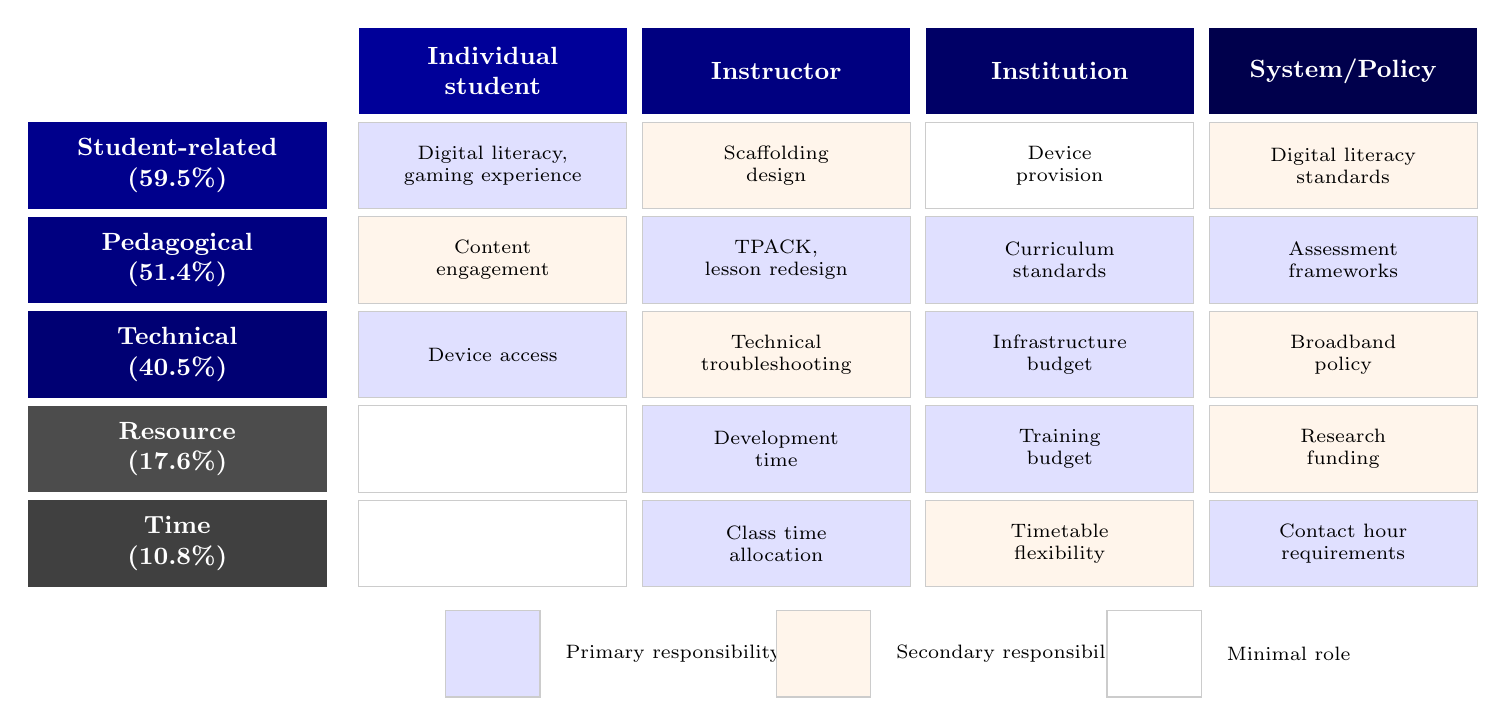
\begin{tikzpicture}[
  hdr/.style={font=\small\bfseries, text=white, minimum height=1.1cm,
    minimum width=3.4cm, align=center},
  rhdr/.style={font=\small\bfseries, text=white, minimum height=1.1cm,
    minimum width=3.8cm, align=center, anchor=east},
  cell/.style={rectangle, draw=gray!40, minimum height=1.1cm,
    minimum width=3.4cm, align=center, font=\scriptsize},
  prim/.style={cell, fill=blue!12},
  sec/.style={cell, fill=orange!8},
  min/.style={cell, fill=white},
]

% Column headers
\node[hdr, fill=blue!60!black] at (0, 0) {Individual\\student};
\node[hdr, fill=blue!50!black] at (3.6, 0) {Instructor};
\node[hdr, fill=blue!40!black] at (7.2, 0) {Institution};
\node[hdr, fill=blue!30!black] at (10.8, 0) {System/Policy};

% Row 1: Student-related (59.5%)
\node[rhdr, fill=blue!55!black] at (-2.1, -1.2) {Student-related\\(59.5\%)};
\node[prim] at (0, -1.2) {Digital literacy,\\gaming experience};
\node[sec] at (3.6, -1.2) {Scaffolding\\design};
\node[min] at (7.2, -1.2) {Device\\provision};
\node[sec] at (10.8, -1.2) {Digital literacy\\standards};

% Row 2: Pedagogical/Curriculum (51.4%)
\node[rhdr, fill=blue!50!black] at (-2.1, -2.4) {Pedagogical\\(51.4\%)};
\node[sec] at (0, -2.4) {Content\\engagement};
\node[prim] at (3.6, -2.4) {TPACK,\\lesson redesign};
\node[prim] at (7.2, -2.4) {Curriculum\\standards};
\node[prim] at (10.8, -2.4) {Assessment\\frameworks};

% Row 3: Technical (40.5%)
\node[rhdr, fill=blue!45!black] at (-2.1, -3.6) {Technical\\(40.5\%)};
\node[prim] at (0, -3.6) {Device access};
\node[sec] at (3.6, -3.6) {Technical\\troubleshooting};
\node[prim] at (7.2, -3.6) {Infrastructure\\budget};
\node[sec] at (10.8, -3.6) {Broadband\\policy};

% Row 4: Resource (17.6%)
\node[rhdr, fill=gray!60!black] at (-2.1, -4.8) {Resource\\(17.6\%)};
\node[min] at (0, -4.8) {};
\node[prim] at (3.6, -4.8) {Development\\time};
\node[prim] at (7.2, -4.8) {Training\\budget};
\node[sec] at (10.8, -4.8) {Research\\funding};

% Row 5: Time (10.8%)
\node[rhdr, fill=gray!50!black] at (-2.1, -6.0) {Time\\(10.8\%)};
\node[min] at (0, -6.0) {};
\node[prim] at (3.6, -6.0) {Class time\\allocation};
\node[sec] at (7.2, -6.0) {Timetable\\flexibility};
\node[prim] at (10.8, -6.0) {Contact hour\\requirements};

% Legend
\node[prim, minimum width=1.2cm] at (0, -7.4) {};
\node[font=\scriptsize, anchor=west] at (0.8, -7.4) {Primary responsibility};
\node[sec, minimum width=1.2cm] at (4.2, -7.4) {};
\node[font=\scriptsize, anchor=west] at (5.0, -7.4) {Secondary responsibility};
\node[min, minimum width=1.2cm] at (8.4, -7.4) {};
\node[font=\scriptsize, anchor=west] at (9.2, -7.4) {Minimal role};

\end{tikzpicture}%
}% end resizebox
\caption{Implementation barrier--stakeholder responsibility matrix. The most frequently reported barriers (student-related, pedagogical) require systemic responses, while the most frequently \textit{addressed} barriers (technical) are tractable at the individual level --- revealing a response mismatch in the literature.}
\label{fig:barrier-stakeholder-matrix}
\end{figure}


\begin{figure}[htbp]
\centering
\resizebox{0.95\textwidth}{!}{%
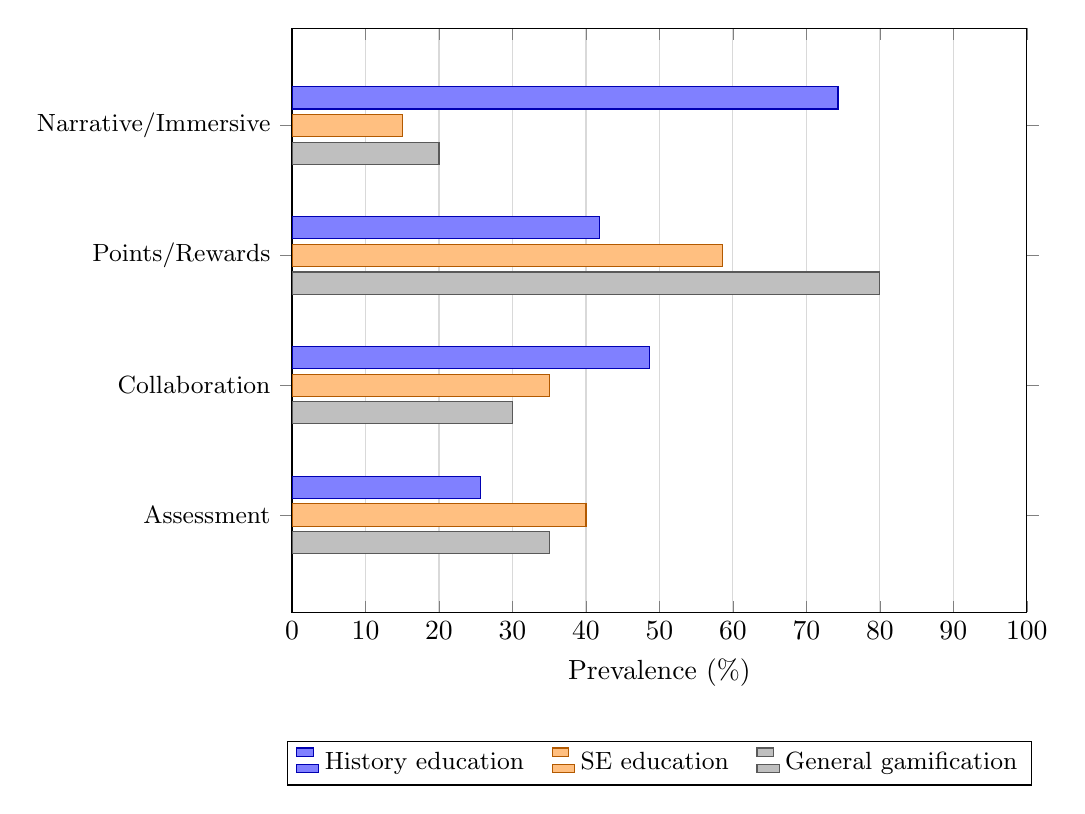
\begin{tikzpicture}
\begin{axis}[
    xbar,
    width=0.9\textwidth,
    height=9cm,
    xlabel={Prevalence (\%)},
    symbolic y coords={
      {Assessment},
      {Collaboration},
      {Points/Rewards},
      {Narrative/Immersive}
    },
    ytick=data,
    y tick label style={font=\small, anchor=east},
    bar width=8pt,
    xmin=0, xmax=100,
    enlarge y limits=0.25,
    xmajorgrids=true,
    ymajorgrids=false,
    grid style={gray!30},
    legend style={
      at={(0.5,-0.22)},
      anchor=north,
      legend columns=3,
      font=\small,
      /tikz/every even column/.append style={column sep=8pt},
    },
    reverse legend,
]
% General gamification (plotted first = bottom bar in each group)
\addplot[fill=gray!50, draw=gray!70!black] coordinates {
  (35,{Assessment})
  (30,{Collaboration})
  (80,{Points/Rewards})
  (20,{Narrative/Immersive})
};
% SE education
\addplot[fill=orange!50, draw=orange!70!black] coordinates {
  (40,{Assessment})
  (35,{Collaboration})
  (58.6,{Points/Rewards})
  (15,{Narrative/Immersive})
};
% History education (plotted last = top bar in each group)
\addplot[fill=blue!50, draw=blue!70!black] coordinates {
  (25.7,{Assessment})
  (48.6,{Collaboration})
  (41.9,{Points/Rewards})
  (74.3,{Narrative/Immersive})
};
\addlegendentry{General gamification}
\addlegendentry{SE education}
\addlegendentry{History education}
\end{axis}
\end{tikzpicture}%
}
\caption{Comparison of game design element prevalence across three educational domains. History education exhibits an inverted profile: experiential elements (narrative, immersion) dominate over reward elements (points), reversing the pattern observed in software engineering education and general gamification.}
\label{fig:domain-element-comparison}
\end{figure}


\begin{figure}[!h]
\centering
\resizebox{\textwidth}{!}{%
\begin{tikzpicture}[
  instbox/.style={rounded corners=6pt, thick, minimum width=6.0cm, minimum height=8.0cm, align=center},
  iheader/.style={font=\small\bfseries, align=center},
  isubt/.style={font=\scriptsize, align=center, text=gray!60!black},
  iitem/.style={font=\scriptsize, align=left},
  linkbox/.style={rounded corners=4pt, fill=yellow!15, draw=yellow!60, thick,
    minimum width=3.8cm, minimum height=4.0cm, align=center},
  botbox/.style={rounded corners=3pt, thick, minimum width=4.5cm, minimum height=0.9cm,
    font=\scriptsize, align=center},
]

% === MRQS box (left) ===
\node[instbox, draw=green!50!black, fill=green!12] (mrqs) at (-5.0, 0) {};
\node[iheader, text=green!50!black] at (-5.0, 3.5) {MRQS};
\node[isubt] at (-5.0, 2.8) {Reporting quality};
\node[isubt] at (-5.0, 2.2) {10 binary items};
\node[isubt] at (-5.0, 1.7) {Codable from data};

\node[iitem, text width=4.8cm] at (-5.0, -0.3) {%
  \textbf{M1} Sample size reported\\
  \textbf{M2} $n \geq 30$\\
  \textbf{M3} Control group\\
  \textbf{M4} Validated instruments\\
  \textbf{M5} Effect sizes\\
  \textbf{M6} Pre-post design\\
  \textbf{M7} Inferential statistics\\
  \textbf{M8} Explicit definition\\
  \textbf{M9} Theoretical framework\\
  \textbf{M10} Limitations discussed
};

% === Adapted ROBIS box (right) ===
\node[instbox, draw=orange!50!black, fill=orange!12] (robis) at (5.0, 0) {};
\node[iheader, text=orange!50!black] at (5.0, 3.5) {Adapted ROBIS};
\node[isubt] at (5.0, 2.8) {Risk of bias};
\node[isubt] at (5.0, 2.2) {3 domains $\times$ 2 questions};
\node[isubt] at (5.0, 1.7) {Judgment-based};

\node[iitem, text width=4.8cm] at (5.0, -0.1) {%
  \textbf{D1} Participant selection\\
  \hspace{1em}Q1: Selection criteria\\
  \hspace{1em}Q2: Representativeness\\[6pt]
  \textbf{D2} Data collection\\
  \hspace{1em}Q3: Instrument validity\\
  \hspace{1em}Q4: Analysis methods\\[6pt]
  \textbf{D3} Interpretation\\
  \hspace{1em}Q5: Conclusion consistency\\
  \hspace{1em}Q6: Limitations discussed
};

% === Center overlap zone ===
\node[linkbox] (overlap) at (0, 0) {};
\node[font=\scriptsize\bfseries, text=yellow!50!black] at (0, 1.6) {Inter-linkages};

\node[font=\scriptsize, align=center] at (0, 0.7) {%
  M4 $\longleftrightarrow$ Q3\\[2pt]
  {\tiny (instrument validation)}};

\node[font=\scriptsize, align=center] at (0, -0.4) {%
  M10 $\longleftrightarrow$ Q6\\[2pt]
  {\tiny (limitations)}};

\node[font=\tiny, text=gray!60!black, align=center] at (0, -1.5) {Same construct,\\different assessment};

% Connecting arrows
\draw[thick, green!50!black, -{Stealth[length=4pt]}] (-1.9, 0.7) -- (-1.05, 0.7);
\draw[thick, orange!50!black, -{Stealth[length=4pt]}] (1.9, 0.7) -- (1.05, 0.7);
\draw[thick, green!50!black, -{Stealth[length=4pt]}] (-1.9, -0.4) -- (-1.05, -0.4);
\draw[thick, orange!50!black, -{Stealth[length=4pt]}] (1.9, -0.4) -- (1.05, -0.4);

% === Bottom distinction boxes ===
\node[botbox, draw=green!50!black, fill=green!8] at (-5.0, -4.8) {``Is it reported?''\\(binary: 0/1)};
\node[botbox, draw=orange!50!black, fill=orange!8] at (5.0, -4.8) {``Is it adequate?''\\(judgment: low/high/unclear)};

% Arrows from main boxes to bottom boxes
\draw[thick, green!50!black, -{Stealth[length=4pt]}] (-5.0, -4.0) -- (-5.0, -4.3);
\draw[thick, orange!50!black, -{Stealth[length=4pt]}] (5.0, -4.0) -- (5.0, -4.3);

\end{tikzpicture}%
}% end resizebox
\caption{Complementarity of the MRQS and adapted ROBIS instruments. The MRQS assesses reporting completeness (binary presence/absence), while the adapted ROBIS assesses risk of bias (evaluative judgment). Two item--question pairs (M4/Q3, M10/Q6) target the same construct from different assessment perspectives, enabling comparison of reporting quality and methodological risk (see Section~\ref{sec:mrqs-framework}).}
\label{fig:mrqs-robis-complementarity}
\end{figure}


% --- Chapter 1 Section 1.3 (MRQS) supplementary tables ---

\begin{table}[!h]
\centering
\caption{Definitional practices across gamification systematic reviews. The present study's 14.9\% explicit definition rate is lower than rates reported in broader gamification reviews, reflecting the disciplinary composition of the history education corpus. A critical distinction applies: ``citing a definition'' (common) differs from ``providing an operational definition'' (rare) (see Section~\ref{sec:def-quality}).}
\label{tab:cross-domain-definitions}
\small
\begin{tabular}{@{}p{3.5cm}p{2.5cm}cp{3cm}p{3cm}@{}}
\toprule
Review & Domain & $N$ & Definition metric & Finding \\
\midrule
Present study \cite{Korniienko2025mrqs} & History education & 74 & Explicit definition provided & 14.9\% \\
Hamari et al.\ \cite{Hamari2014} & General gamification & 24 & Referenced Deterding \cite{Deterding2011} & $\sim$75\% cited \\
Koivisto \& Hamari \cite{KoivistoHamari2019} & General gamification & 365 & Referenced canonical definition & Majority cited \\
Seaborn \& Fels \cite{SEABORN201514} & General gamification & 32 & Provided operational definition & $\sim$50\% estimated \\
Sailer \& Homner \cite{SailerHomner2020} & Learning gamification & 38 & Defined gamification & Not reported \\
Dichev \& Dicheva \citeauthor{DichevDicheva2017}~\cite{DichevDicheva2017} & Education gamification & 51 & Noted ``definitional confusion'' & Systemic \\
\bottomrule
\end{tabular}
\end{table}

\begin{table}[!h]
\centering
\caption{Statistical power analysis at representative sample sizes from the 74-study corpus. Minimum detectable effect sizes ($d$) are computed for two-group comparisons at 80\% power and $\alpha = .05$ (two-tailed). The \citeauthor{Kraft2020}~\cite{Kraft2020} recalibrated benchmark of $d = 0.20$ for ``large'' effects in scalable educational interventions contextualises the severe underpowering of the typical study (see Section~\ref{sec:detailed-bias}).}
\label{tab:power-analysis}
\small
\begin{tabular}{@{}lccccc@{}}
\toprule
Design & Total $n$ & $n$/group & Detectable $d$ & Kraft & Status \\
\midrule
Two-group & 34 (median) & 17 & $\approx$0.98 & 0.20 & Severely underpowered \\
Two-group & 50 (75th pctl) & 25 & $\approx$0.81 & 0.20 & Severely underpowered \\
Two-group & 128 & 64 & $\approx$0.50 & 0.20 & Underpowered \\
Two-group & 394 (adequate) & 197 & $\approx$0.20 & 0.20 & Adequately powered \\
Pre-post paired & 34 (median) & 34 paired & $\approx$0.49 & 0.20 & Underpowered \\
\bottomrule
\end{tabular}
\end{table}

\begin{table}[!h]
\centering
\caption{Evidence gap map: number of studies by outcome domain and study design in the 74-study corpus. Gap severity reflects both the volume and quality of available evidence. Critical gaps in historical thinking, long-term retention, and cost-effectiveness represent the highest-priority targets for future research (see Section~\ref{sec:research-priorities}).}
\label{tab:evidence-gap-map}
\small
\begin{tabular}{@{}lcccccp{2.8cm}@{}}
\toprule
\textbf{Outcome domain} & \textbf{Case/Qual} & \textbf{Pre--post} & \textbf{Quasi-exp} & \textbf{RCT} & \textbf{Total} & \textbf{Gap severity} \\
\midrule
Engagement / Motivation & 10 & 26 & 18 & 1 & 55 & Moderate \\
Knowledge acquisition   &  4 & 22 & 18 & 1 & 45 & Moderate \\
Attitudes / Satisfaction &  8 & 20 & 11 & 0 & 39 & High \\
Historical thinking     &  5 &  5 &  4 & 0 & 14 & Critical \\
Long-term retention     &  0 &  2 &  0 & 0 &  2 & Critical \\
Cost-effectiveness      &  0 &  0 &  0 & 0 &  0 & Total absence \\
\bottomrule
\end{tabular}

\smallskip
\noindent\textit{Note.} Cell counts derived from the 74-study MRQS corpus \cite{Korniienko2025mrqs}. Studies measuring multiple outcomes appear in multiple rows; column totals therefore exceed~74. ``Pre--post'' denotes single-group designs without comparison conditions. The single RCT employed a qualitative-dominant mixed-methods design and does not provide quantitative effect estimates for the engagement or knowledge domains.
\end{table}

\begin{table}[!h]
\centering
\caption{Distribution of studies by country of application ($n=74$; some studies report multiple countries). Taiwan's dominance reflects sustained national EdTech policy (MOST/NSC funding) and established game-based learning research groups (see Section~\ref{sec:evidence-base}).}
\label{tab:country-distribution}
\small
\begin{tabular}{lclc}
\hline
\textbf{Country} & \textbf{n} & \textbf{Country} & \textbf{n} \\
\hline
Taiwan & 13 & United States & 11 \\
Malaysia & 9 & Indonesia & 8 \\
Canada & 6 & Greece & 5 \\
Spain & 4 & United Kingdom & 3 \\
Sweden & 3 & Italy & 3 \\
Poland & 3 & Peru & 2 \\
Netherlands & 2 & Pakistan & 1 \\
Japan & 1 & Tunisia & 1 \\
Saudi Arabia & 1 & Chile & 1 \\
Portugal & 1 & Turkey & 1 \\
Denmark & 1 & Australia & 1 \\
China (Hong Kong) & 1 & Ireland & 1 \\
Austria & 1 & Germany & 1 \\
China & 1 & & \\
\hline
\end{tabular}
\end{table}

% --- Chapter 2 supplementary figures ---

\begin{figure}[!h]
\centering

\includegraphics[width=0.6\textwidth]{posibnyk_1_nmt_structure.jpg}
\caption{Gamified NMT structure poster (``Know the Test'') illustrating the test structure through a gamified infographic format (see Section~\ref{sec:organisation}).}
\label{fig:nmt-structure}
\end{figure}

\input{figures/digcomp_alignment_matrix}

\begin{figure}[!h]
\centering

\includegraphics[width=0.7\textwidth]{posibnyk_4_visual_sources.jpg}
\caption{Course material: visual source identification exercise featuring historical portraits of key Ukrainian figures (Mazepa, Hrushevskyi, Petliura, Stalin) with associated artifacts (see Section~\ref{sec:organisation}).}
\label{fig:visual-sources}
\end{figure}

\begin{figure}[!h]
\centering

\includegraphics[width=0.75\textwidth]{hlg_threejs.png}
\caption{Chronobiy (``Time Slayer'') game: a timeline-sorting battle where players arrange historical events chronologically to defeat period-specific opponents. Built with Three.js for 3D visual effects (see Section~\ref{sec:gamification-design}).}
\label{fig:hlg-threejs}
\end{figure}

\begin{figure}[!h]
\centering

\includegraphics[width=0.75\textwidth]{hlg_solitaire.png}
\caption{Historical solitaire: Cossack era card game with four thematic categories (Hetman politics, Military campaigns, Cultural life, International relations) requiring chronological sorting within each theme (see Section~\ref{sec:gamification-design}).}
\label{fig:hlg-solitaire}
\end{figure}

\begin{figure}[!h]
\centering

\includegraphics[width=0.65\textwidth]{hlg_bobble.png}
\caption{Bobble Shooter: Imperial period game where coloured bubbles represent historical categories (Culture, Politics, Economy, Military affairs) and players match three or more to clear the field (see Section~\ref{sec:gamification-design}).}
\label{fig:hlg-bobble}
\end{figure}

\begin{figure}[!h]
\centering

\includegraphics[width=0.55\textwidth]{hlg_accessibility.png}
\caption{Inclusivity settings panel of the HistoryLikeGame platform: theme switching (dark/light), font size scaling (A/A+/A++), reduced motion, and high-contrast mode. Settings persist via \texttt{localStorage} and respect system-level user preferences (see Section~\ref{sec:gamification-design}).}
\label{fig:hlg-accessibility}
\end{figure}

\begin{figure}[!h]
\centering
\resizebox{\textwidth}{!}{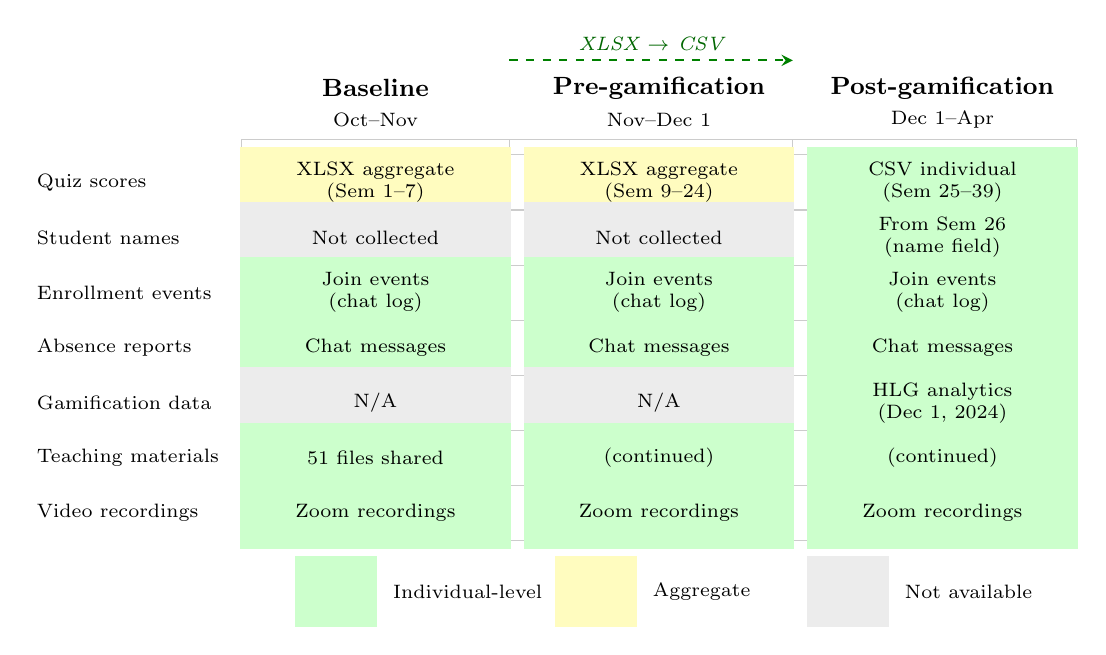
\begin{tikzpicture}[
  font=\small,
  cell/.style={minimum width=3.4cm, minimum height=0.9cm, align=center, font=\scriptsize, text width=3.2cm},
  indiv/.style={cell, fill=green!20},
  aggr/.style={cell, fill=yellow!25},
  nodata/.style={cell, fill=gray!15},
  header/.style={minimum width=3.4cm, minimum height=0.5cm, align=center, font=\small\bfseries, fill=white},
  subheader/.style={minimum width=3.4cm, minimum height=0.4cm, align=center, font=\scriptsize, fill=white},
  rowlabel/.style={minimum width=2.8cm, minimum height=0.7cm, align=left, font=\scriptsize, text width=2.6cm},
  phasearr/.style={->, >=stealth, thick, green!50!black, dashed}
]

% Column positions: row labels at x=1.0, columns at x=4.0, 7.6, 11.2
\def\cola{4.0}
\def\colb{7.6}
\def\colc{11.2}
\def\rowx{1.0}

% Column headers (two rows: title + date range)
\node[header] at (\cola, 0.2) {Baseline};
\node[subheader] at (\cola, -0.2) {Oct--Nov};
\node[header] at (\colb, 0.2) {Pre-gamification};
\node[subheader] at (\colb, -0.2) {Nov--Dec 1};
\node[header] at (\colc, 0.2) {Post-gamification};
\node[subheader] at (\colc, -0.2) {Dec 1--Apr};

% Row labels and horizontal lines
\foreach \y/\rowlbl in {
  -1.0/Quiz scores,
  -1.7/Student names,
  -2.4/Enrollment events,
  -3.1/Absence reports,
  -3.8/Gamification data,
  -4.5/Teaching materials,
  -5.2/Video recordings%
}{
  \node[rowlabel] at (\rowx, \y) {\rowlbl};
  \draw[gray!40] (2.3, \y+0.35) -- (12.9, \y+0.35);
}
\draw[gray!40] (2.3, -0.45) -- (12.9, -0.45);
\draw[gray!40] (2.3, -5.55) -- (12.9, -5.55);

% Vertical dividers
\foreach \x in {2.3, 5.7, 9.3, 12.9}{
  \draw[gray!40] (\x, -0.45) -- (\x, -5.55);
}

% Quiz scores row
\node[aggr] at (\cola, -1.0) {XLSX aggregate\\(Sem 1--7)};
\node[aggr] at (\colb, -1.0) {XLSX aggregate\\(Sem 9--24)};
\node[indiv] at (\colc, -1.0) {CSV individual\\(Sem 25--39)};

% Student names row
\node[nodata] at (\cola, -1.7) {Not collected};
\node[nodata] at (\colb, -1.7) {Not collected};
\node[indiv] at (\colc, -1.7) {From Sem 26\\(name field)};

% Enrollment row
\node[indiv] at (\cola, -2.4) {Join events\\(chat log)};
\node[indiv] at (\colb, -2.4) {Join events\\(chat log)};
\node[indiv] at (\colc, -2.4) {Join events\\(chat log)};

% Absence row
\node[indiv] at (\cola, -3.1) {Chat messages};
\node[indiv] at (\colb, -3.1) {Chat messages};
\node[indiv] at (\colc, -3.1) {Chat messages};

% Gamification row
\node[nodata] at (\cola, -3.8) {N/A};
\node[nodata] at (\colb, -3.8) {N/A};
\node[indiv] at (\colc, -3.8) {HLG analytics\\(Dec 1, 2024)};

% Materials row
\node[indiv] at (\cola, -4.5) {51 files shared};
\node[indiv] at (\colb, -4.5) {(continued)};
\node[indiv] at (\colc, -4.5) {(continued)};

% Video row
\node[indiv] at (\cola, -5.2) {Zoom recordings};
\node[indiv] at (\colb, -5.2) {Zoom recordings};
\node[indiv] at (\colc, -5.2) {Zoom recordings};

% Data format evolution arrow — placed above column headers
\draw[phasearr] (5.7, 0.55) -- node[above, font=\scriptsize\itshape, green!40!black] {XLSX $\to$ CSV} (9.3, 0.55);

% Legend
\node[indiv, minimum width=1.0cm, text width=0.8cm] at (3.5, -6.2) {};
\node[font=\scriptsize, anchor=west] at (4.1, -6.2) {Individual-level};
\node[aggr, minimum width=1.0cm, text width=0.8cm] at (6.8, -6.2) {};
\node[font=\scriptsize, anchor=west] at (7.4, -6.2) {Aggregate};
\node[nodata, minimum width=1.0cm, text width=0.8cm] at (10.0, -6.2) {};
\node[font=\scriptsize, anchor=west] at (10.6, -6.2) {Not available};

\end{tikzpicture}
}
\caption{Data collection matrix: data types (rows) mapped to study phases (columns). Green = individual-level data, yellow = aggregate data, grey = not available. The XLSX-to-CSV transition marks the shift from aggregate to individual-level quiz score data (see Section~\ref{sec:organisation}).}
\label{fig:data-matrix}
\end{figure}

\begin{figure}[!h]
\centering
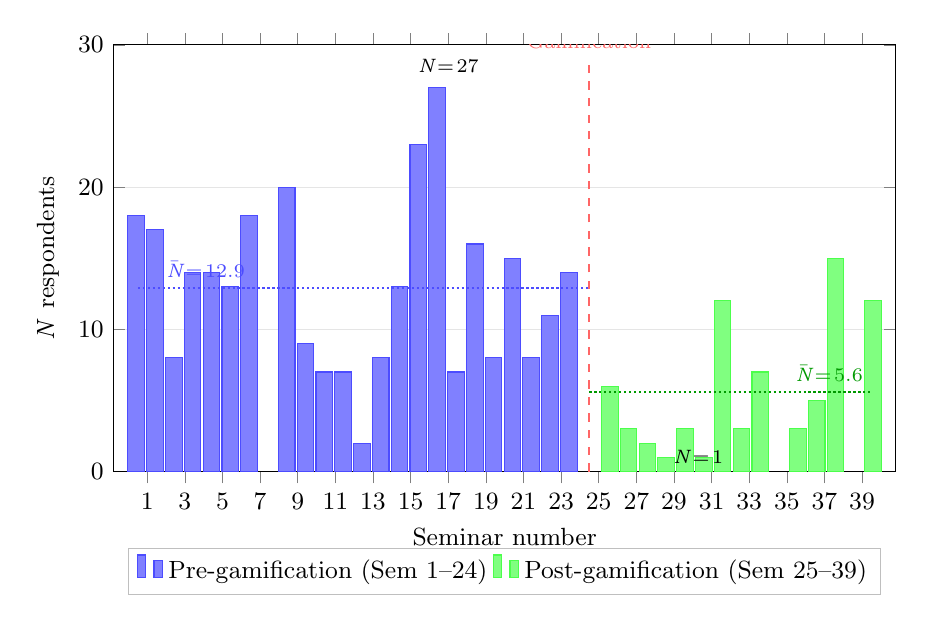
\begin{tikzpicture}
\begin{axis}[
  ybar,
  width=0.95\textwidth,
  height=7cm,
  bar width=6pt,
  ylabel={\textit{N} respondents},
  xlabel={Seminar number},
  ymin=0, ymax=30,
  xtick={1,3,5,7,9,11,13,15,17,19,21,23,25,27,29,31,33,35,37,39},
  xmin=0, xmax=40,
  enlarge x limits=0.02,
  legend style={at={(0.5,-0.18)}, anchor=north, legend columns=2, font=\small, draw=gray!50},
  ymajorgrids=true,
  grid style={gray!20},
  tick label style={font=\small},
  label style={font=\small},
]

% Pre-gamification bars (blue)
\addplot[fill=blue!50, draw=blue!70] coordinates {
  (1,18) (2,17) (3,8) (4,14) (5,14) (6,13) (7,18)
  (9,20) (10,9) (11,7) (12,7) (13,2) (14,8) (15,13)
  (16,23) (17,27) (18,7) (19,16) (20,8) (21,15) (22,8) (23,11) (24,14)
};

% Post-gamification bars (green)
\addplot[fill=green!50, draw=green!70] coordinates {
  (25,6) (26,3) (27,2) (28,1) (29,3) (30,1)
  (31,12) (32,3) (33,7) (35,3) (36,5) (37,15) (39,12)
};

\legend{Pre-gamification (Sem 1--24), Post-gamification (Sem 25--39)}

% Gamification boundary
\draw[dashed, thick, red!60] (axis cs:24.5,0) -- (axis cs:24.5,29)
  node[above, font=\scriptsize, red!60] {Gamification};

% Period mean lines
\draw[densely dotted, blue!70, thick] (axis cs:0.5,12.9) -- (axis cs:24.5,12.9)
  node[pos=0.15, above, font=\scriptsize, blue!70] {$\bar{\textit{N}}\!=\!12.9$};
\draw[densely dotted, green!60!black, thick] (axis cs:24.5,5.6) -- (axis cs:39.5,5.6)
  node[pos=0.85, above, font=\scriptsize, green!60!black] {$\bar{\textit{N}}\!=\!5.6$};

% Annotations
\node[font=\scriptsize, above, yshift=2pt] at (axis cs:17,27) {$\textit{N}\!=\!27$};
\node[font=\scriptsize, right, xshift=3pt] at (axis cs:28,1) {$\textit{N}\!=\!1$};

\end{axis}
\end{tikzpicture}

\caption{Number of respondents per seminar quiz. Blue bars = pre-gamification period (Seminars~1--24, $\bar{\textit{N}}\!=\!12.9$); green bars = post-gamification period (Seminars~25--39, $\bar{\textit{N}}\!=\!5.6$). Dashed vertical line marks the gamification introduction (December~1, 2024) (see Section~\ref{sec:organisation}).}
\label{fig:respondent-progression}
\end{figure}

\begin{figure}[!h]
\centering

\includegraphics[width=0.65\textwidth]{posibnyk_6_digital_platforms.jpg}
\caption{Digital platform integration poster (``Plug In. Log On.''): the ecosystem of digital tools used in the course, orienting students toward self-directed learning across multiple platforms as a lifelong learning competence (see Section~\ref{sec:wartime-context}).}
\label{fig:digital-platforms}
\end{figure}

% --- Chapter 3 supplementary figures ---

\begin{figure}[!h]
\centering
\begin{tikzpicture}
\pgfplotstableread{figures/full_course_comparison_data.csv}\datatable
\begin{axis}[
    width=0.95\textwidth,
    height=7cm,
    xlabel={Seminar number},
    ylabel={Mean score (\%)},
    ymin=0, ymax=110,
    xmin=0, xmax=41,
    grid=major,
    grid style={gray!30},
    xtick={1,5,10,15,20,25,30,35,40},
    legend style={at={(0.02,0.98)}, anchor=north west, font=\small},
]
% Shaded regions
\fill[blue!8] (axis cs:0,0) rectangle (axis cs:24.5,110);
\fill[green!8] (axis cs:24.5,0) rectangle (axis cs:41,110);
\node[font=\scriptsize, text=blue!60!black] at (axis cs:12,105) {Pre-gamification};
\node[font=\scriptsize, text=green!60!black] at (axis cs:33,105) {Post-gamification};
\draw[dashed, gray, thick] (axis cs:24.5,0) -- (axis cs:24.5,110);

% Mean line
\addplot[blue!70!black, thick, mark=*, mark size=1.5pt] table[x=seminar, y=mean_pct] {\datatable};
\addlegendentry{Mean \%}
\end{axis}
\end{tikzpicture}
\caption{Full-course mean score comparison with pre-gamification (Seminars 1--24) and post-gamification (Seminars 25--39) regions (see Section~\ref{sec:baseline}).}
\label{fig:full-comparison}
\end{figure}

\begin{figure}[!h]
\centering
\begin{tikzpicture}
\pgfplotstableread{figures/score_distribution_data.csv}\datatable
\begin{axis}[
    width=0.95\textwidth,
    height=7cm,
    xlabel={Seminar number},
    ylabel={Mean score (\%) $\pm$ SD},
    ymin=0, ymax=120,
    xmin=0, xmax=41,
    grid=major,
    grid style={gray!30},
    xtick={1,5,10,15,20,25,30,35,40},
]
\addplot[ybar, fill=blue!40, draw=blue!70!black, bar width=0.6,
    error bars/.cd, y dir=both, y explicit]
    table[x=seminar, y=mean_pct, y error=sd_pct] {\datatable};
\end{axis}
\end{tikzpicture}
\caption{Mean score distribution by seminar ($\pm$ SD) across the full course (see Section~\ref{sec:baseline}).}
\label{fig:distribution}
\end{figure}

\begin{figure}[!h]
\centering
\begin{tikzpicture}
\pgfplotstableread{figures/modular_control_data.csv}\datatable
\begin{axis}[
    width=0.85\textwidth,
    height=6cm,
    xlabel={Modular control},
    ylabel={Mean score (\%)},
    ymin=0, ymax=110,
    axis y line*=left,
    grid=major,
    grid style={gray!30},
    xtick={1,2,3,4,5,6,7},
    legend style={at={(0.3,-0.28)}, anchor=north, font=\small, draw=gray!50},
]
% Mean line with error bars
\addplot[blue, thick, mark=o, mark size=2pt,
    error bars/.cd, y dir=both, y explicit]
    table[x=mc, y=mean_pct, y error=sd_pct] {\datatable};
\addlegendentry{Mean \% $\pm$ SD}
\end{axis}

\begin{axis}[
    width=0.85\textwidth,
    height=6cm,
    axis y line*=right,
    axis x line=none,
    ylabel={Number of respondents},
    ymin=0, ymax=30,
    xtick={1,2,3,4,5,6,7},
    legend style={at={(0.7,-0.28)}, anchor=north, font=\small, draw=gray!50},
]
\addplot[ybar, fill=green!20, draw=green!50!black, bar width=8pt, opacity=0.6] table[x=mc, y=N] {\datatable};
\addlegendentry{\textit{N} respondents}
\end{axis}
\end{tikzpicture}
\caption{Modular control progression: mean score (\%) with SD error bars and number of respondents (see Section~\ref{sec:baseline}).}
\label{fig:mc-progression}
\end{figure}

\begin{figure}[!h]
\centering
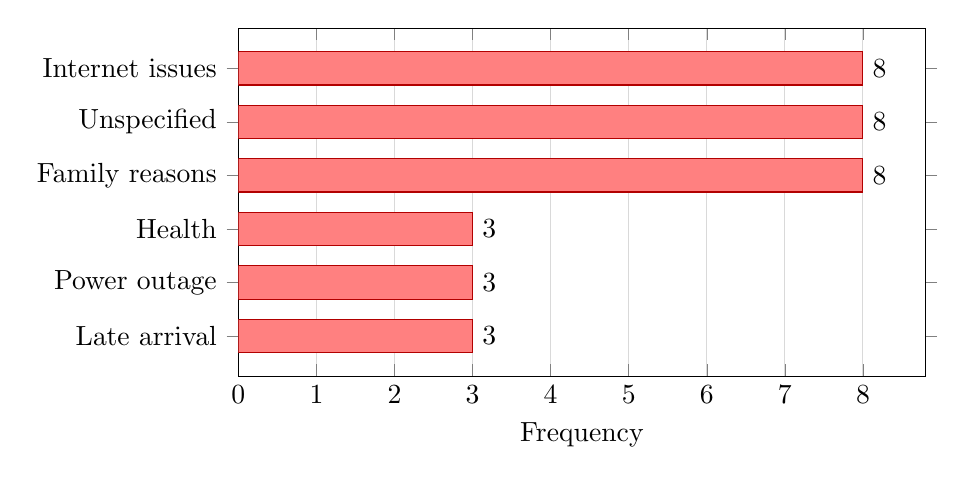
\begin{tikzpicture}
\begin{axis}[
    width=0.85\textwidth,
    height=6cm,
    xbar,
    xlabel={Frequency},
    symbolic y coords={{Late arrival}, {Power outage}, {Health}, {Family reasons}, {Unspecified}, {Internet issues}},
    ytick=data,
    nodes near coords,
    nodes near coords align={horizontal},
    bar width=12pt,
    xmin=0,
    enlarge y limits=0.15,
    xmajorgrids=true,
    ymajorgrids=false,
    grid style={gray!30},
]
\addplot[fill=red!50, draw=red!70!black] coordinates {(3,{Late arrival}) (3,{Power outage}) (3,{Health}) (8,{Family reasons}) (8,{Unspecified}) (8,{Internet issues})};
\end{axis}
\end{tikzpicture}
\caption{Distribution of absence reasons reflecting wartime education conditions (see Section~\ref{sec:baseline}).}
\label{fig:absence}
\end{figure}

\begin{figure}[!h]
\centering
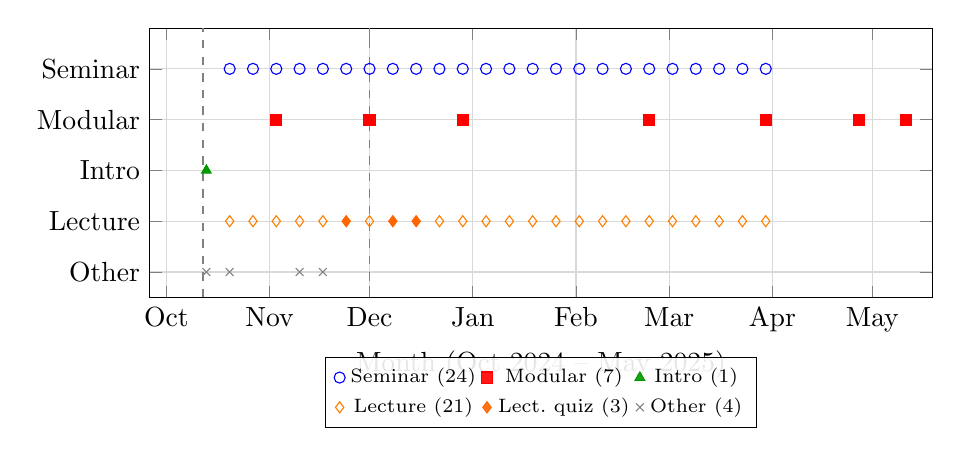
\begin{tikzpicture}
\begin{axis}[
    width=0.95\textwidth,
    height=5cm,
    xlabel={Month (Oct 2024 -- May 2025)},
    xticklabels={Oct, Nov, Dec, Jan, Feb, Mar, Apr, May},
    xtick={0,31,61,92,123,151,182,212},
    yticklabels={Other, Lecture, Intro, Modular, Seminar},
    ytick={0,1,2,3,4},
    grid=major,
    grid style={gray!30},
    legend style={at={(0.5,-0.22)}, anchor=north, font=\scriptsize, legend columns=3, fill=white, fill opacity=0.9, draw opacity=1, text opacity=1},
    ymin=-0.5, ymax=4.8,
    xmin=-5, xmax=230,
]
\addplot[only marks, mark=o, mark size=2pt, blue] coordinates {(19,4) (26,4) (33,4) (40,4) (47,4) (54,4) (61,4) (68,4) (75,4) (82,4) (89,4) (96,4) (103,4) (110,4) (117,4) (124,4) (131,4) (138,4) (145,4) (152,4) (159,4) (166,4) (173,4) (180,4)};
\addlegendentry{Seminar (24)}
\addplot[only marks, mark=square*, mark size=2pt, red] coordinates {(33,3) (61,3) (89,3) (145,3) (180,3) (208,3) (222,3)};
\addlegendentry{Modular (7)}
\addplot[only marks, mark=triangle*, mark size=2pt, green!60!black] coordinates {(12,2)};
\addlegendentry{Intro (1)}
\addplot[only marks, mark=diamond, mark size=2pt, orange] coordinates {(19,1) (26,1) (33,1) (40,1) (47,1) (61,1) (82,1) (89,1) (96,1) (103,1) (110,1) (117,1) (124,1) (131,1) (138,1) (145,1) (152,1) (159,1) (166,1) (173,1) (180,1)};
\addlegendentry{Lecture (21)}
\addplot[only marks, mark=diamond*, mark size=2pt, orange!80!red] coordinates {(54,1) (68,1) (75,1)};
\addlegendentry{Lect.\ quiz (3)}
\addplot[only marks, mark=x, mark size=2pt, gray] coordinates {(12,0) (19,0) (40,0) (47,0)};
\addlegendentry{Other (4)}
\draw[dashed, gray] (axis cs:11,-0.5) -- (axis cs:11,4.8) node[above, font=\tiny, text=gray] {Start};
\draw[dashed, gray] (axis cs:61,-0.5) -- (axis cs:61,4.8) node[above, font=\tiny, text=gray] {Gamification};
\end{axis}
\end{tikzpicture}

\caption{Complete course assessment timeline (October 2024 -- May 2025) (see Section~\ref{sec:baseline}).}
\label{fig:timeline}
\end{figure}

\begin{figure}[!h]
\centering
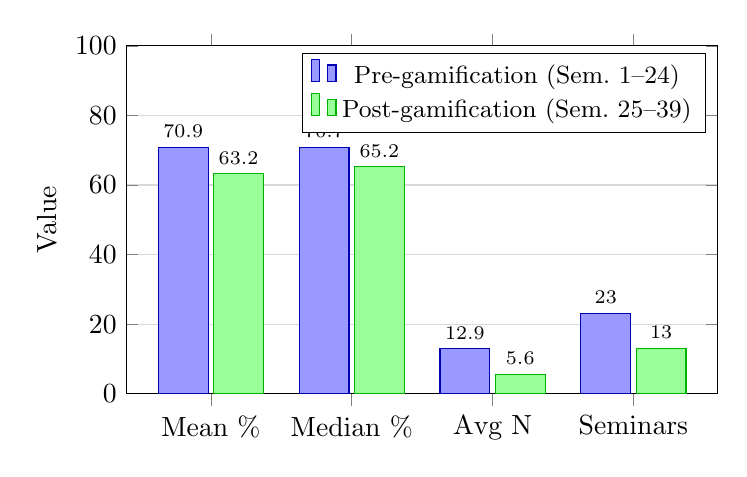
\begin{tikzpicture}
\begin{axis}[
    width=0.75\textwidth,
    height=6cm,
    ybar,
    bar width=18pt,
    ylabel={Value},
    symbolic x coords={Mean \%, Median \%, Avg N, Seminars},
    xtick=data,
    ymin=0, ymax=100,
    legend style={at={(0.98,0.98)}, anchor=north east, font=\small},
    nodes near coords,
    nodes near coords style={font=\scriptsize},
    enlarge x limits=0.2,
    xmajorgrids=false,
    ymajorgrids=true,
    grid style={gray!30},
]
\addplot[fill=blue!40, draw=blue!70!black] coordinates {
    ({Mean \%},70.9)
    ({Median \%},70.7)
    ({Avg N},12.9)
    ({Seminars},23)
};
\addlegendentry{Pre-gamification (Sem.\ 1--24)}

\addplot[fill=green!40, draw=green!70!black] coordinates {
    ({Mean \%},63.2)
    ({Median \%},65.2)
    ({Avg N},5.6)
    ({Seminars},13)
};
\addlegendentry{Post-gamification (Sem.\ 25--39)}
\end{axis}
\end{tikzpicture}
\caption{Summary comparison of pre-gamification (Seminars 1--24) and post-gamification (Seminars 25--39) periods (see Section~\ref{sec:baseline}).}
\label{fig:pre-post}
\end{figure}

\label{last_page}
